% ---------------------------------------------------
% ----- Main document of the template
% ----- for Bachelor-, Master thesis and class papers
% ---------------------------------------------------
%  Created by C. Müller-Birn on 2012-08-17, CC-BY-SA 3.0.
%  Last upadte: C. Müller-Birn 2015-11-27
%  Freie Universität Berlin, Institute of Computer Science, Human Centered Computing. 

\documentclass[pdftex,a4paper,12pt,DIV=calc,BCOR5mm,ngerman,twoside,smallheadings,titlepage]{scrbook}   
% ----- weitere Optionen 
%draft,			% Entwurfsmodus zum Anzeigen zu leerer/voller Boxen 
%DIV=calc
%DIV12,			% Seitengröße (siehe Koma Skript Dokumentation !) 
%BCOR5mm,		% Zusätzlicher Rand auf der Innenseite 
%twoside,		% Seitenränder werden an doppelseitig angepasst 
%fleqn,			% Formeln werden linksbündig (und nicht zentriert) angezeigt 
%titlepage,		% Titel wird in einer 'titlepage' Umgebung gesetzt 
%bigheadings,	% Große Überschriften (normal, small-headings) 
%halfparskip-	% Absatz wird nicht eingerückt, dafür aber um eine halbe Zeile nach unten gerückt
%
%---------------------------------------------------
%----- Packages
%---------------------------------------------------
%
\usepackage[]{pythontex}
\usepackage[T1]{fontenc} 
\usepackage[utf8]{inputenc}
\usepackage[english]{babel}  
\usepackage{ae} 
\usepackage{bibgerm}    

\usepackage{fancyhdr} % Define simple headings 
\usepackage{xcolor}
\usepackage{url}
\usepackage{listings}
%\usepackage{vmargin} % Adjust margins in a simple way
%
\usepackage{amsmath}
%
\usepackage[pdftex]{graphicx}  
\usepackage{hyperref} % turn all your internal references into hyperlinks
%\usepackage[pdfstartview=FitH,pdftitle={<<Titel der Arbeit>>}, pdfauthor={<<Autor>>}, pdfkeywords={<<Schlüsselwörter>>}, pdfsubject={<<Titel der Arbeit>>}, colorlinks=true, linkcolor=black, citecolor=black, urlcolor=black, hypertexnames=false, bookmarksnumbered=true, bookmarksopen=true, pdfborder = {0 0 0}]{hyperref}
%
% table settings 
\usepackage{booktabs}  
\usepackage{tabularx}  
\usepackage{rotating}
\usepackage{longtable}
\usepackage{pdflscape}
\usepackage{multirow} %multi row
\usepackage{rotating} %for rotating table
% custom imports

\usepackage{tikz}
\usetikzlibrary{shapes,arrows}
\usepackage{amssymb}
\usepackage{longtable}
\usepackage{float}
%
%---------------------------------------------------
%----- PDF and document setup
%---------------------------------------------------
%
\hypersetup{
	pdftitle={Developing interpretability techniques for unsupervised topic modelling},  % please, add the title of your thesis
    pdfauthor={Tim Korjakow},   % please, add your name
    pdfsubject={Bachelor thesis, Institute of Computer Science, Freie Universität Berlin}, % please, select the type of this document
    pdfstartview={FitH},    % fits the width of the page to the window
    pdfnewwindow=true, 		% links in new window
    colorlinks=false,  		% false: boxed links; true: colored links
    linkcolor=red,          % color of internal links
    citecolor=green,        % color of links to bibliography
    filecolor=magenta,      % color of file links
    urlcolor=cyan           % color of external links
}
% 
%---------------------------------------------------
%----- Customize page size
%---------------------------------------------------
\usepackage[top=3cm,right=3cm,bottom=4cm,left=4cm]{geometry}    
%
%---------------------------------------------------
%----- Customize header and footer\pagestyle{fancy} 
%---------------------------------------------------
\pagestyle{fancy}

\fancyhf{}  % delete all existing header formating

\fancyhead[LE]{\leftmark}  % represent the current chapter heading in uppercase
\renewcommand{\chaptermark}[1]{ % adapt the shown chapter name: show it in lower case and with chapter number 
\markboth{\thechapter.\ #1}{}}   

\fancyhead[RO]{\rightmark}   % % represent the current section heading in uppercase 
\renewcommand{\sectionmark}[1]{% adapt the shown section name: show it in lower case and with section number 
\markboth{\thesection.\ #1}{}}

\definecolor{tim}{rgb}  {0.6, 0.1, 0.4}
\newcommand{\tk}[1]{\textcolor{tim}{[\textbf{TK:} #1]}} % add author comments

\renewcommand{\headrulewidth}{0pt} % remove lines from header
\renewcommand{\footrulewidth}{0pt} % remove lines from header

\fancyfoot{} % delete all existing footer formating
\fancyfoot[LE,RO]{\thepage} % put page number on the left on even page and right on odd page
%
%---------------------------------------------------      
%----- Settings for word separation  
%---------------------------------------------------      
% Help for separation (from package babel, section 22)):
% In german package the following hints are additionally available:
% "- = an explicit hyphen sign, allowing hyphenation in the rest of the word
% "| = disable ligature at this position. (e.g., Schaf"|fell)
% "~ = for a compound word mark without a breakpoint (e.g., bergauf und "~ab)
% "= = for a compound word mark with a breakpoint, allowing hyphenation in the composing words
% "" = like "-, but producing no hyphen sign (e.g., und/""oder)
%
% Describe separation hints here:
\hyphenation{
% Pro-to-koll-in-stan-zen
% Ma-na-ge-ment  Netz-werk-ele-men-ten
% Netz-werk Netz-werk-re-ser-vie-rung
% Netz-werk-adap-ter Fein-ju-stier-ung
% Da-ten-strom-spe-zi-fi-ka-tion Pa-ket-rumpf
% Kon-troll-in-stanz
}
%
%---------------------------------------------------
%----- Restricting including files   
%---------------------------------------------------
% Only files listed here will be included in the PDF document!
% In order to only partially translate the document, for example for bug-fixing, 
% it might be useful to comment out some of the documents.
\includeonly{
../chapters/title/title,
../chapters/declaration/declaration,
../chapters/abstract/abstract_en,
../chapters/abstract/abstract_de,
../chapters/preface/preface,
../chapters/introduction/introduction,
../chapters/literature_analysis/literature_analysis,
../chapters/implementation/implementation,
../chapters/validation/validation,
../chapters/conclusion/conclusion,
../chapters/appendix/appendix
}

%%%%%%%%%%%%%%%%%%%%%%%%%%%%%%%%%%%%%%%%%%%%%%%%%%%%%%
% The content part of the documentent starts here! %%
%%%%%%%%%%%%%%%%%%%%%%%%%%%%%%%%%%%%%%%%%%%%%%%%%%%%%%

\begin{document}
%---------------------------------------------------
%----- Listing and color definition   
%---------------------------------------------------
\definecolor{red}{rgb}{.8,.1,.2}
\definecolor{blue}{rgb}{.2,.3,.7}
\definecolor{lightyellow}{rgb}{1.,1.,.97}
\definecolor{gray}{rgb}{.7,.7,.7}
\definecolor{darkgreen}{rgb}{0,.5,.1}
\definecolor{darkyellow}{rgb}{1.,.7,.3}
\lstloadlanguages{C++,[Objective]C}
\lstset{
		escapeinside={§§}{§§},
        basicstyle=\ttfamily\footnotesize\mdseries,
        columns=fullflexible,% typewriter font look better with fullflex
        keywordstyle=\bfseries\color{blue},
%		identifierstyle=\bfseries,
        commentstyle=\color{darkgreen},      
        stringstyle=\color{red},
        numbers=left,
        numberstyle=\ttfamily\scriptsize\color{gray},
%       stepnumber=5,
%       numberfirstline=true,
        breaklines=true,
%		prebreak=\\,
        showstringspaces=true,
        tabsize=4,
        captionpos=b,
%		framexrightmargin=-.2\textwidth,
        float=htb,
		frame=tb,
		frameshape={RYR}{n}{n}{RYR},
		rulecolor=\color{darkyellow},
        xleftmargin=15pt,
        xrightmargin=4pt,
        aboveskip=\bigskipamount,
        belowskip=\bigskipamount,
		backgroundcolor=\color{lightyellow},
		extendedchars=true,
       	belowcaptionskip=15pt
}

%---------------------------------------------------
%----- Title and declaration   
%---------------------------------------------------
\pagenumbering{alph} % even though, these page numbers are not visible there are necessary to have unique page numbers 
% ---------------------------------------------------
% ----- Title page of the template
% ----- for Bachelor-, Master thesis and class papers
% ---------------------------------------------------
%  Created by C. Müller-Birn on 2012-08-17, CC-BY-SA 3.0.
%  Freie Universität Berlin, Institute of Computer Science, Human Centered Computing. 
%
\begin{titlepage}

\title{
\includegraphics[width=0.6\textwidth]{pics/FU_logo.pdf}\\
{\small Bachelorarbeit am Institut für Informatik der Freien Universität Berlin}\\
{\small Human-Centered Computing (HCC)}\\
[6ex]
{\LARGE Comparing interpretability techniques for unsupervised topic modeling}}

\author{
{\emph{\normalsize Tim Korjakow}}\\
{\normalsize Matrikelnummer: 372862}\\
{\normalsize Email: tim.korjakow@campus.tu-berlin.de}\\ 
[18ex]   
{\normalsize Betreuer: Jesse Jonas Benjamin} \\
{\normalsize Betreuerin und Erstgutachterin: Prof. Dr. C. Müller-Birn} \\
{\normalsize Zweitgutachter: Prof. Dr. K. Müller}}
\vspace{6ex}
\date{\normalsize Berlin, 08.08.2019}
 
\maketitle  

\end{titlepage}
% ---------------------------------------------------
% ----- Declaration of the template
% ----- for Bachelor-, Master thesis and class papers
% ---------------------------------------------------
%  Created by C. Müller-Birn on 2012-08-17, CC-BY-SA 3.0.
%  Freie Universität Berlin, Institute of Computer Science, Human Centered Computing. 
%
\pagestyle{empty}

\subsection*{Eidesstattliche Erklärung}

Ich versichere hiermit an Eides Statt, dass diese Arbeit von niemand anderem als meiner Person verfasst worden ist. Alle verwendeten Hilfsmittel wie Berichte, Bücher, Internetseiten oder ähnliches sind im Literaturverzeichnis angegeben, Zitate aus fremden Arbeiten sind als solche kenntlich gemacht. Die Arbeit wurde bisher in gleicher oder ähnlicher Form keiner anderen Prüfungskommission vorgelegt und auch nicht veröffentlicht.
\par\bigskip  
\noindent Berlin, den \today

\vspace{1.2cm}

\noindent <Name>  

\cleardoublepage

%---------------------------------------------------
%----- Abstracts in English and German   
%---------------------------------------------------

% ---------------------------------------------------
% ----- Abstract (English) of the template
% ----- for Bachelor-, Master thesis and class papers
% ---------------------------------------------------
%  Created by C. Müller-Birn on 2012-08-17, CC-BY-SA 3.0.
%  Freie Universität Berlin, Institute of Computer Science, Human Centered Computing. 
%
\pagestyle{empty}

\subsection*{Abstract}

<Please summarize your thesis in a brief but meaningful way (about one page). Include in your abstract the topic of this thesis, important contents, results of your research and an evaluation of your results.>

\cleardoublepage

% ---------------------------------------------------
% ----- Abstract (German) of the template
% ----- for Bachelor-, Master thesis and class papers
% ---------------------------------------------------
%  Created by C. Müller-Birn on 2012-08-17, CC-BY-SA 3.0.
%  Freie Universität Berlin, Institute of Computer Science, Human Centered Computing. 
%
\pagestyle{empty}

\subsection*{Zusammenfassung}

<Hier sollten Sie eine kurze, aussagekräftige Zusammenfassung (ca. eine Seite) Ihrer Arbeit geben, welche das Thema der Arbeit, die wichtigsten Inhalte, die Arbeitsergebnisse und die Bewertung der Ergebnisse umfasst.> 

\cleardoublepage 
                                          
%---------------------------------------------------
%----- Directories   
%---------------------------------------------------

\frontmatter 
\pagenumbering{roman}

\tableofcontents
\setcounter{tocdepth}{3}   % reduce the included sections in the table of content

\listoffigures
\listoftables

%---------------------------------------------------
%----- Main part
%---------------------------------------------------
\mainmatter
\pagenumbering{arabic} 
\pagestyle{fancy} 

%% ---------------------------------------------------
% ----- Preface of the template
% ----- for Bachelor-, Master thesis and class papers
% ---------------------------------------------------
%  Created by C. Müller-Birn on 2012-08-17, CC-BY-SA 3.0.
%  Freie Universität Berlin, Institute of Computer Science, Human Centered Computing. 
%
\chapter*{Vorwort}
\label{chap:preface}

\section*{Allgemeine Hinweise zur Erstellung einer Abschlussarbeit}

\begin{itemize}
	\item Beachten Sie, dass diese Vorlage für einen zweiseitigen Ausdruck angelegt wurde.  
	\item Über die Papierqualität können Sie entscheiden, aber wir empfehlen aber Seiten mit wichtigen, farbigen Grafiken auch in Farbe auszudrucken und dabei ein höherwertiges Papier zu verwenden. 
	\item Bitte stimmen Sie mit dem Betreuer Ihrer Arbeit auch den Zweitgutachter ab. Die Anfrage des Zweitgutachters erfolgt von Ihnen. Es ist an dieser Stelle sinnvoll, die Anfrage mit einer kurzen Zusammenfassung der Arbeit zu stellen.  
	\item Bitte beachten Sie, dass Sie Ihre Abschlussarbeit mit einer Klebebindung versehen, eine Ringbindung ist nicht erwünscht. 
\end{itemize} 

% ---------------------------------------------------
% ----- Introduction of the template
% ----- for Bachelor-, Master thesis and class papers
% ---------------------------------------------------
%  Created by C. Müller-Birn on 2012-08-17, CC-BY-SA 3.0.
%  Last upadte: C. Müller-Birn 2015-11-27 
%  Freie Universität Berlin, Institute of Computer Science, Human Centered Computing. 
%
\chapter{Thematic Introduction and Motivation}
\label{chap:introduction}

\section{Project IKON}

This thesis has a direct application in a project which tries to explore potentials for knowledge transfer activities at a research museum. Project \textit{IKON} was started in cooperation with the German Natural History Museum in Berlin which houses more than 300 scientists, PhD students and other staff \cite{Team2018}. With that size of scientific staff the institution is a global player in research on evolution and biodiversity \cite{IntroducingMuseumFur}. Despite its importance in the research landscape, the museum is challenged with a lack of shared knowledge across working groups and organizational structures such as departments. In interviews researchers from the project were able to trace these problems back to the very intricate and complex layout of rooms and halls in the building which was originally constructed in 1810 \cite{140JahreAltes2018}. In order to mitigate this problem \autoref{pic:IKON-clusterview} shows one of the main deliverables of \textit{IKON} - a ML-driven data visualization which follows the path of knowledge at this research museum from its creation in projects over knowledge transfer activities, where multiple projects exchange their findings, to the final target group. Potentials for knowledge exchange are made explicit by visualizing projects not in the predefined taxonomy of the museum, but instead in semantic relation to each other. This is accomplished by running all project abstracts through a topic modeling process consisting of four major components, as seen in \autoref{pic:general_topic_extraction_pipeline}. 

\section{Topic modeling}

A generic topic modeling pipeline consists of four steps: 
\begin{enumerate}
	\item Document embedding
	\item Topic extraction
	\item Classification of documents
	\item Reduction into 2D
\end{enumerate}

Given an unlabeled corpus $C = \{D_1, ..., D_n\}$ consisting of $n$ documents $D_i = (t_1, ..., t_m)$, which in turn consists of a sequence of $m$ strings, also called tokens or words, the document embedding step assigns to each document a vector $v_D \in \mathbb{R}^e, e \in \mathbb{N}^+$. Semantically similar documents should also be closer in the embedded vector space with respect to a given distance measure than documents which are semantically not related. Therefore this step transforms a corpus into a matrix $(v_1, ..., v_n) \in \mathbb{R}^{e \times n}$.

Consuming the output from the previous step the topic extraction tries to uncover $k$ latent structures. We call these structures \textit{topics}. Mathematically speaking a topic is a probability distribution over a fixed set of input features. \cite{liuOverviewTopicModeling2016} These features can correspond to tokens, as it is the case in the later discussed Tfidf-BOW embedding, but this does not have to be the case. Therefore this step transforms the corpus from the embedding space of dimensionality $e \times n$, where each document is described as linear combination of features, to the latent space of dimensionality $k \times n$, where each document is described as a linear combination of latent topics. Since most often $k < e$ holds true, this can also be seen as a form of dimensionality reduction, which is again a form of feature extraction.

Using the document vectors in the latent space each document is assigned a label. This may happen in a supervised way if there are labels available for training purposes, but in most cases an unsupervised classification, also known as clustering, is used to group the documents.

Finally in order to visualize the high dimensional distribution of documents in the latent space another dimensionality reduction is used to project the documents to 2D.

\begin{figure}[t]
	\centering
	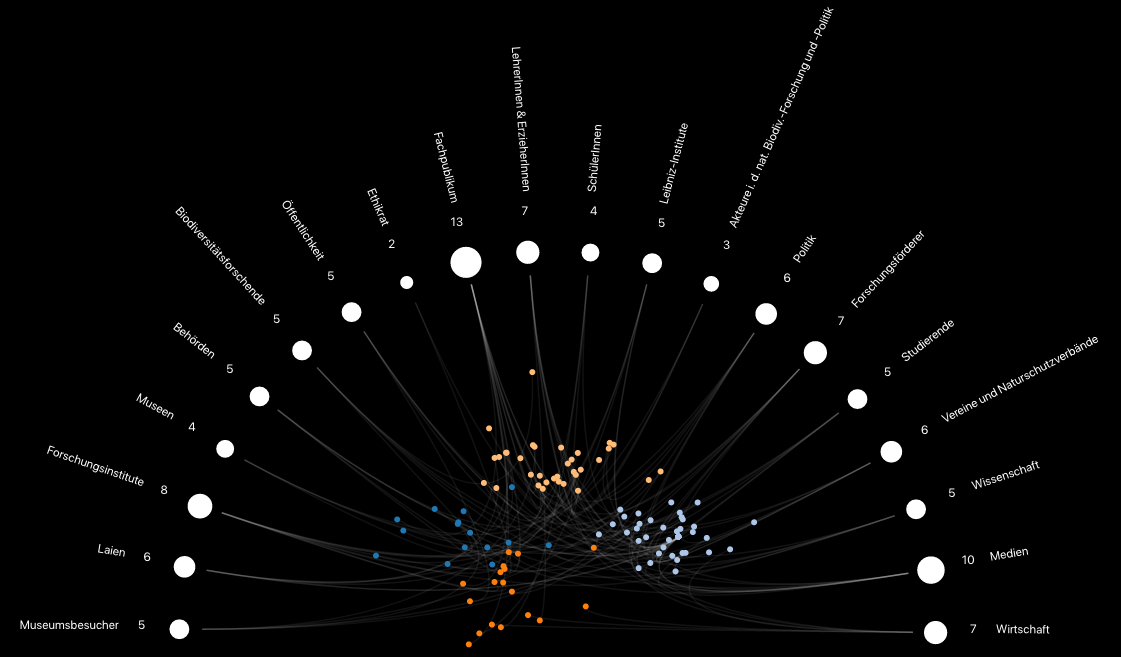
\includegraphics[width=400px]{../chapters/introduction/graphics/ikon-clusterview}
	\caption{\label{pic:IKON-clusterview} Screenshot of the cluster view of the IKON visualization}
\end{figure}

% Define block styles
\tikzstyle{decision} = [diamond, draw, fill=blue!20, 
text width=4.5em, text badly centered, node distance=3cm, inner sep=0pt]
\tikzstyle{block} = [rectangle, draw, fill=blue!20, 
text width=6.5em, text centered, rounded corners, minimum height=4em]
\tikzstyle{line} = [draw, -latex']
\tikzstyle{cloud} = [draw, ellipse,fill=red!20, node distance=3cm,
minimum height=2em]
\usetikzlibrary{decorations.text}

\begin{figure}[t]
	\centering
	\begin{tikzpicture}[node distance = 4cm, auto]
	% Place nodes
	\node [block] (emb) {Document embedding};
	%\node [cloud, left of=emb] (expert) {expert};
	%\node [cloud, right of=emb] (system) {system};
	\node [block, right of=emb] (topic) {Topic extraction};
	\node [block, right of=topic, above of=topic] (cluster) {Classification of documents};
	\node [block, right of=topic, below of=topic] (2D) {Reduction into 2D};
	% Draw edges
	\path [line] (emb) -- (topic);
	\path [line] (topic) -- (cluster);
	\path [line] (topic) -- (2D);
	%\path [line] (identify) -- (evaluate);
	%\path [line] (update) |- (identify);
	%\path [line,dashed] (system) |- (evaluate);
	\end{tikzpicture}
	\caption{\label{pic:general_topic_extraction_pipeline} Components of a general topic extraction pipeline}
\end{figure}

Each component in \autoref{pic:general_topic_extraction_pipeline} comes with its own set of parameters which influence the results generated by the pipeline. Therefore the researchers from project IKON hypothesize, based in first interviews and conceptual work, that the museum's staff, as non-technical experts without knowledge of the capabilities and shortcomings of the models used in topic modeling, will have a hard time interpreting and understanding the output generated by the pipeline. 

In order to lay the groundwork for this thesis and understand the challenges which scientists face while interacting with the visualization I carried out an exploratory workshop with the researchers from project \textit{IKON}. In the beginning I asked them which kind of hardships they, based on their past experiences and interviews, hypothesize during the interaction between user and visualization. Followed by an explanation of \autoref{pic:general_topic_extraction_pipeline} we discussed how these challenges may correlate with goals and questions. Following a description of the key questions each question was categorized according to the pipeline step, as seen in \autoref{tab:overview_viz_questions}, which may contribute information in order to support the user in answering his question.

\begin{table}
	\centering
	\begin{tabular}{ c | c }
		\hline 
		Question & Applicable pipeline component \\ \hline
		How does the research landscape look like \\ and on what kind of topics are prominent? & Topic Extraction \\ \hline
		What does a cluster mean? & Classification \\ \hline
		What does the distance between \\ clusters/projects mean? & Topic Extraction / Reduction into 2D \\ \hline
		How similar are two projects/clusters? & Topic Extraction \\
		\hline
	\end{tabular}
	\caption{\label{tab:overview_viz_questions} Table showing the sourced questions and the pipeline step which could provide an answer}
\end{table} 

\section{Interpretability}

In the same workshop we also developed a way of structuring commonly used terminology in the field of explainability/interpretability research, where terms explainability and interpretability are commonly used as synonyms. Our notion builds upon the findings of Miller and Lipton, which concluded that, interpretability as term has become an ill-defined objective \cite{liptonMythosModelInterpretability2016a} for research and development in ML algorithms since there is no widely agreed upon definition of it. This leads to a very fragmented nature of the field. Furthermore Miller et al. \cite{millerExplainableAIBeware2017} support this point by conducting a literature study and uncovering that interpretability research is rarely influenced by insights from the humanities, especially connected fields as explainability or causality research.

Therefore the researchers from project IKON propose that the context in which interpretation is performed is essential to the outcome of the interpretative process. In this discussion the term 'context' considers the situational context of the interaction between user and system as well as the historical experiences of the user. They introduce a relational model in which users posses a set of \textit{a priori} preferred explanation strategies (e.g. comparing two entities) given the context of the interaction and their previous experiences. As a consequence of having this preferred set, they only consider a specific subset of all possible types of explanations as valid. Interpretability techniques on the other hand are conditioned in regard to an algorithmic system, e.g. a specific model or class of models. These techniques can be described by algorithms and deliver concrete explanations given a model and a model output. Therefore a interpretability technique serves as the missing link between high-level explanation strategies, an algorithmic system and explanations.
 

\begin{figure}[t]
	\centering
	\begin{tikzpicture}[node distance = 6cm, auto]
	% Place nodes
	\node [block] (strat) {Explanation strategy};
	\node [block, right of=strat] (expl) {Explanation};
	\node [block, below of=strat] (alg) {Algorithmic system};
	\node [block, below of=expl] (int) {Interpretability technique};
	% Draw edges
	\path [line,dashed,
	postaction={decorate},
	decoration={text along path,
		text=requires,
		text align={left indent={0.2\dimexpr\pgfdecoratedpathlength\relax}}
	}] 
	(strat) -- (expl);
	
	\path [line,
	postaction={decorate},
	decoration={text along path,
		text=instantiates,
		text align={left indent={0.2\dimexpr\pgfdecoratedpathlength\relax}}
	}] 
	(int) -- (strat);
	
	\path [line,
	postaction={decorate},
	decoration={text along path,
		text=produces,
		text align={left indent={0.2\dimexpr\pgfdecoratedpathlength\relax}}
	}]
	(int) -- (expl);
	
	\path [line,
	postaction={decorate},
	decoration={text along path,
		text=conditions,
		text align={left indent={0.2\dimexpr\pgfdecoratedpathlength\relax}}
	}] 
	(alg) -- (int);
	\end{tikzpicture}
	\caption{\label{pic:interpretability_relational} Relational model showing the interplay of explanation strategies, interpretability techniques and explanations}
\end{figure}

\section{Working plan}
In order to research how these interpretability techniques could be applied in project IKON, I will conduct the following three steps:

\begin{enumerate}
	\item Since I as a developer did not possess an exhaustive list of techniques to enhance explainability for unsupervised NLP models exist, a thorough and reproducible literature analysis on the status of XAI research in the field of NLP according to Petersen et al. \cite{petersenSystematicMappingStudies2008a} is going to be conducted. This should result in a number of papers which are, according to the process, good representatives of the literature base and therefore also of current research efforts. A quantitative analysis of these papers should summarize occurring XAI methods and categorize them according to an applicable categorization. 
	
	\item The currently existing topic extraction pipeline can be generalized into the following four components: document embedding, dimensionality reduction into a topic space, clustering and another dimensionality reduction into 2D. Based on the results of the previous step for each component either a directly applicable method (e.g. a clustering algorithm) from a paper or a model which supports most collected methods (e.g. a neural network for document embedding) is chosen and implemented. Since the new pipeline should capture at least as much information as the old one, each component will be quantitatively accessed according to applicable measures e.g. (\cite{roderExploringSpaceTopic2015a}). This is necessary to ensure that one is actually interpreting existing and captured semantic relations and not random artifacts generated by the various methods.
	
	\item A full user study would normally be necessary to assess how the implemented methods may support a non-technical expert in interpreting the results of the pipeline, but in order to keep the volume of this thesis in a feasible frame I will resort to a cognitive walkthrough from the point of view of a researcher from the national natural history museum.
	Since ensuring robustness in such qualitative tests is always a concern, information from previous interviews with domain experts from the museum will be used to derive meaningful tasks. The walkthrough should show how the implemented techniques may help with answering the initially sourced questions from step 1.
\end{enumerate}


% !TeX root = ../main/thesis_main.tex
% ---------------------------------------------------
% ----- Chapters of the template
% ----- for Bachelor-, Master thesis and class papers
% ---------------------------------------------------
%  Created by C. Müller-Birn on 2012-08-17, CC-BY-SA 3.0.
%  Freie Universität Berlin, Institute of Computer Science, Human Centered Computing.
% 
% Set up python path for all used code in this session and track all external files
\begin{pycode}
import sys
sys.path.insert(0, '../chapters/literature_analysis/code/')
# track code
pytex.add_dependencies('../chapters/literature_analysis/code/analyze_top_publishers.py')
pytex.add_dependencies('../chapters/literature_analysis/code/analyze_time_dist.py')
pytex.add_dependencies('../chapters/literature_analysis/code/analyze_top_keywords.py')
pytex.add_dependencies('../chapters/literature_analysis/code/analyze_mappings.py')
# track data
pytex.add_dependencies('../chapters/literature_analysis/data/meta_search.csv')
pytex.add_dependencies('../chapters/literature_analysis/data/stage1.bib')
pytex.add_dependencies('../chapters/literature_analysis/code/params.json')
pytex.add_dependencies('../chapters/literature_analysis/data/mapping.xlsx')
\end{pycode}

\chapter{Literature mapping study}
\label{chap:literature_analysis}

\section{Motivation}

In order to access current methods in the fast-moving field of interpretability research in machine learning in a reproducible and structured fashion I will conduct a literature mapping study according to Petersen et. al \cite{petersenSystematicMappingStudies}, which consists of a number of sequential steps which should result in a representative corpus and an analysis using it.

\section{Methodology}

The process from Petersen et al. is augmented by further steps in order to tailor it to the existing use case and consists of the following seven procedures:
\begin{enumerate}
	
	\item Definition of research questions:
	
	The overall process starts by defining clear questions which should guide the development of the whole literature mapping study and subsequently the result as well. Since I am interested in gaining an overview over the existing interpretability techniques for NLP, I chose the following questions:
	
	\begin{enumerate}
		\item What categories of explainability techniques are mentioned in the corpus?
		\item What kind of models are enhanced by explainability techniques?
		\item Which techniques are applicable to results produced by the pipeline or the pipeline itself?
	\end{enumerate}
	
	\item Construction of a search string:
	
	Based on the questions one is able to gather a set of key words which are most relevant to the field which is analyzed. Each word is augmented by synonyms which are concatenated with boolean OR operators and several of these synonymous groups are again connected via logical ANDs. Applying this method to the previously found questions yields the following search string:
	
\begin{pycode}
import json
with open('../chapters/literature_analysis/code/params.json') as json_file:
	params = json.load(json_file)
	search_string = ' AND '.join( '( ' + ' OR '.join([ f'"{item}"' for item in ors]) + ' )' for ors in params["stage1"])
	
	print(r"\textit{")
	print(search_string)
	print(r"}")
\end{pycode}
	
	
	\item Analysis of the main publishers using a meta search and the search string:
	
	Due to the presumed distributed nature of interpretability research it is not easy to pinpoint the main publishers of scientific articles. In order to mitigate this, a pre-search in the meta-search engine 'Google Scholar' is conducted. It should be noted at this point that any biases which are apparent in the meta search engine therefore apply to this analysis as well. One can see in \autoref{fig:top_publisher} that the main publishers are respectivly Arxiv, IEEE, Springer and ACM. Since all of these publishers are mainly focused on publications in computer science, mathematics and engineering, this speaks in favor of the hypothesis that the majority of the research is still very technical and research from social sciences rarely influences it. Even though Arxiv is not a credible publisher per se, it seems like the research community uses it as the first place to publish work and therefore it should not be excluded in this analysis. 
	
\begin{pycode}
from analyze_top_publishers import show_top_publishers
show_top_publishers('../chapters/literature_analysis/data/meta_search.csv', 'top_publisher')
\end{pycode}

	\item Sourcing of publications in scientific databases:
	
	Based on the insights from the previous step each of the main publisher's databases is scraped using the search string and their respective 'advanced search' interfaces or their APIs. Since most searches result in more than 1000 publications only the top 100 results ordered by the relevance scoring of the database are taken into account. These publications then form the corpus which is the basis for further analysis.
	
	\item Intermediate assessment of the corpus:
	
	Looking at the distribution of tags in \autoref{fig:top_keywords} it is apparent that the chosen keywords represent the field well. There are no tags in the first 5 entries which are not constructable by the query.
	Plotting the distribution of publishing dates of the papers from the corpus in \autoref{fig:time_dist} reveals that the first publications were already written in 1980, while there is a surge of interest and research in the last 4 years. This speaks in favor of the premise that interpretability research is not necessarily a young, but a recently thriving field.
	
\begin{pycode}
from analyze_time_dist import print_time_dist
print_time_dist('../chapters/literature_analysis/data/stage1.bib', 'time_dist')
\end{pycode}

\begin{pycode}
from analyze_top_keywords import print_top_keywords
print_top_keywords('../chapters/literature_analysis/data/stage1.bib', 'top_keywords')
\end{pycode}
	
	\item Definition and application of inclusion and exclusion criteria to narrow down the pool of publications further:
	
	The next step serves as another filtering step enhancing the quality of the hitherto automatic selection by using human decision making. A combination of the guiding questions, which were defined in the beginning of the process and a first pass over the whole corpus, in which I skimmed the papers, gave me a clear set of criteria, as seen in \autoref{tbl:incl_excl}, which can be used to filter the corpus further. In a second pass each paper was evaluated and included in the next step if and only if it satisfied at least one inclusion criterion and none of the exclusion criteria.	In order to support my decision making and minimize the amount of work to classify each paper I developed a Jupyter-based interface, which takes a bibliography and a set of inclusion and exclusion criteria and iterates over all contained publications, shows its title and abstract and allows the user to select criteria which apply. If a closer examination is needed it opens the paper on demand. Furthermore it sorts each publication into either a bibliography for the next stage, a bibliography with rejected publications depending on the applying criteria or a bibliography containing interesting, but not directly relevant literature. I opensourced this framework on \href{https://github.com/wittenator/limap}{GitHub}.
	
	\begin{table}
		\centering
		\begin{tabular}{  p{5cm} | p{5cm} }
			Inclusion criteria & Exclusion criteria  \\ \hline
			
			\begin{itemize}
				\item Reviews the current state of explainability research
				\item Presents a specific method for enhancing explainability for models
			\end{itemize}
			
			&
			
			\begin{itemize}
				\item Is not scientific literature
				\item Does not describe the used explainability method
				\item The publication does not focus on explainability
				\item The described method is neither general, nor focused on NLP
			\end{itemize}
		\end{tabular}
		\caption{\label{tbl:incl_excl} Table showing all used inclusion and exclusion criteria}
	\end{table}
	
	\item Quantitative assessment of the resulting corpus:
	
	In the last step the actual mapping is generated. In another pass I first skimmed and then read each paper and based on that classified each publication and its presented technique in order to answer the initially posed questions. To answer the first question I categorized them according to the proposed categories of Hohman et. al. \cite{hohmanGamutDesignProbe2019}. These categories are not a perfect fit for a thesis dealing with explainability for non-technical experts since it also categorizes techniques according to their mathematical inner workings, but Hohman et al. extended the categories proposed by Lipton \cite{liptonMythosModelInterpretability2016a}, which formulated the starting hypothesis for this thesis and is the closest to a nontechnical assessment of interpretability research I could find. Furthermore each publication was assigned the type of model to which the technique is applicable, the component to which the technique could be applied in the topic extraction pipeline and each paper was classified as either "Theory", "Method", "Study" or "Report". 
	A "Method" paper presents a single explainability technique and demonstrates its impact in an exemplary use case. A "Theory" paper does so as well, but misses a presented application and evaluation. A "Report" on the other hand summarizes and presents multiple techniques. Finally, a "Study" paper shows the results of an interface evaluation which visualizes the output of explainability methods. Publications from the last category are therefore less technical and more concerned with the HCI aspects of explainability techniques and their visualization.
	
	Since most of the overview papers presented a huge amount of techniques which were already covered by the "Method" papers and the corpus was already large, I decided to exclude them from the last mapping step. This reduced the final corpus to a size of 72 publications.

\end{enumerate}

\section{Results}

In order to answer my first question concerning the different kinds of researched explainability 

Mapping the type of paper and the classification according to Gamut each on an axis (\autoref{fig:type_gamut}) shows clearly that there is a trend towards developing methods which explain single decision instances (38 paper). Furthermore most developed methods are tested on real world data (61 paper), but their application in an interface is rarely studied (6 paper). This speaks in favor of the hypothesis that most explainability methods are developed as mathematical theories and influences from HCI are rarely taken into consideration.

\begin{pycode}
from analyze_mappings import print_mapping
print_mapping('../chapters/literature_analysis/data/mapping.xlsx', 'type_gamut', 'Mapping of the type of publication and its Gamut classification', 'Gamut extended', 'Type')
\end{pycode}

The second question was concerned with the type of models which are enhanced by explainability techniques. In \autoref{fig:application_gamut} it is visible that neural architectures (NN, CNN, FNN, RNN, GCNN) dominate the field (40 paper). 19 papers try to explain a given model in an agnostic way as a black box, while a minority of publications deals with the explainability of clustering results, decision trees or linear models.

\begin{pycode}
from analyze_mappings import print_mapping
print_mapping('../chapters/literature_analysis/data/mapping.xlsx', 'application_gamut', 'Mapping of applicability and Gamut classification', 'Gamut extended', 'Applicability')
\end{pycode}

The third mapping in \autoref{fig:pipelinestep_gamut} shows the relation between the applicability of a method in the general topic extraction pipeline and its Gamut classification. Suprisingly, 51\% of the sourced publications are not applicable to the general topic extraction pipeline in any form. The two main reasons why a publication falls into this category is that it either presents a method in a subdomain of NLP which is not directly applicable \cite{goyalTransparentAISystems2016} \cite{itoTextVisualizingNeuralNetwork2018a} or its presented use case and context is too far off in order to be applied \cite{8591457} \cite{gengHumancentricTransferLearning}.
The second biggest category consists of techniques which could be applied to the document classification step using labeled data to train a model. Since any neural network can be used to classify vectorized documents, most of the publications on the "NN" axis in \autoref{fig:application_gamut} fall into this bucket as well. All in all, 18 publications remain which could be applied to an unsupervised topic extraction pipeline. 
The document embedding step could be made interpretable by decomposition, feature importance visualization or by explaining the embedding of single instances. 

Kim et al. \cite{kimStructureDeepNeural2019} decompose a pretrained network and extract simple features which they use as to train a neural network on another task in a transfer learning fashion. The predictions for new tasks can then be described as a combination of these extracted features.

In contrast to that, Zhang et al. \cite{zhangUnsupervisedLearningNeural2018} train another neural network to explain the output of any given neural network in a unsupervised way. They focus on CNNs and utilize the fact that these convolutional layers contain structural information. For each input they are able to disentagle the information from the applied convolutional filters and extract features which can be applied back to the input as masks to show influential parts. Given a document embedding technique, which uses CNNs, and a corpus this explainability technique could be used to highlight influential parts of the input document.

\begin{pycode}
from analyze_mappings import print_mapping
print_mapping('../chapters/literature_analysis/data/mapping.xlsx', 'pipelinestep_gamut', 'Mapping of pipeline step and Gamut classification', 'Gamut extended', 'Pipeline step')
\end{pycode}


% !TeX root = ../main/thesis_main.tex
% ---------------------------------------------------
% ----- Chapters of the template
% ----- for Bachelor-, Master thesis and class papers
% ---------------------------------------------------
%  Created by C. Müller-Birn on 2012-08-17, CC-BY-SA 3.0.
%  Freie Universität Berlin, Institute of Computer Science, Human Centered Computing.
% 
% Set up python path for all used code in this session and track all external files
\begin{pycode}
import sys
sys.path.insert(0, '../chapters/implementation/code/')
# track code

\end{pycode}

\chapter{Implementation}
\label{chap:implementation}

\section{General setup}

In order to ensure that the results of this thesis are usable for further work and research it was one of my priorities to integrate all my code into the existing project as well as possible. Since the IKON project uses a Docker-based microservice architecture to develop and manage their servers, I decided to integrate the Jupyter Notebook, which I used as my main tool for code development and documentation, into this network. Doing this also enabled the Notebook to dynamically fetch data from the Postgres database which serves as the main source of information.
In anticipation of huge computational loads the Docker container was designed to make use of a potential graphic card. That's why I built all my work on top of the official Tensorflow Docker image which comes with all the drivers for NVidia GPUs. The problem with that image is that it either detects a graphic card and suitable drivers and works or it fails in case of no present drivers. For that reason I created a Shell which makes the use of the container easier. By activating a $--gpu$ flag while executing the script, the docker container dynamically selects an image with or without GPU support, starts the Notebook container and the database in a separate network and scans the output of the Notebook container in order to extract the Notebook credentials, which are necessary to access the program via the browser, and opens a browser session once these credentials were found.

\section{Data and Preprocessing}
Since one of the main aims of project IKON is to connect projects semantically instead of by using the rigid taxonomy of the museum, I was able to use the project's abstract which is recorded in the GEPRIS database of the DFG \cite{DFGGEPRIS}. It consists of almost all projects which were supported by the DFG since 2000. Fortunately, another bachelor project before me worked on a scraper which extracted approximately 114.000 projects from the web interface of the database since there is no publicly available API. Each project was characterized by a title, a project abstract in German or English, start and end dates as well as additional meta data like connected institutions or people working in the project.

As one can see in \autoref{pic:gepris_histogram}, there is a peak at word count 3 and one at approximatly 100. The first one corresponds to all projects which do not have descriptions, because they are described with "Keine Zusammenfassung vorhanden". The latter peak on the other hand is produced by projects from a fund which uses the same descriptions for all its projects which are financed through the DFG.

\begin{figure}[t]
	\centering
	\includegraphics[width=400px]{/home/tim/HCC/IKON-backend/src/topicextraction/nlp/plots/histogram}
	\caption{\label{pic:gepris_histogram} Histogram showing the distribution of text lengths in the dataset}
\end{figure}

Removing these peaks in \autoref{pic:gepris_cleaned_histogram} reveals that most texts have an length of 150 words, while also having smaller peaks at ca. 70 and 350 words. The shortest description has a length of one word and the longest  983 words.

\begin{figure}[t]
	\centering
	\includegraphics[width=400px]{/home/tim/HCC/IKON-backend/src/topicextraction/nlp/plots/cleaned_histogram}
	\caption{\label{pic:gepris_cleaned_histogram} Histogram showing the distribution of text lengths in the dataset excluding duplicates and projects without a description}
\end{figure}

Following the advice of Matthew et al. \cite{dennymatthewpennstateuniversity;spirlingarthurnewyorkuniversityReplicationDataText2017} the texts were preprocessed by a P-N-S-W scheme. First punctuation (P) and numbers (N) were removed since sentence boundaries or specific numbers do not bear a lot of information in middle-sized descriptive texts. Following this, according to the categories of Matthew et al., a stemming step (S) is performed, which uses lemmatization to find the lemmas of words by using vocabularies and the context of each word. The last step removes infrequent words without much semantic meaning, commonly known as stopwords (W). Lowercasing and n-gram inclusion were omitted, because casing is an important feature for distinguishing nouns from other word types in the German language, which helps the lemmatization step, and the use of word composition makes most reasonable n-grams in other languages appear as one word in German. 

Until the start of this thesis the pipeline did all this preprocessing using regex-based rules and a lemmatization using the SpaCy lemmatizer. This proved to be a viable option until a corpus size of 5000 since after that point the running time was too long to effectively work with it. Therefore I bundled all the preprocessing operations in a new class called \textit{Datapreprocessor}, which should be able to transform any given query into a preprocessed dataset for the following pipeline steps as well as cache its results. In order to do that I rewrote the preprocessing steps and integrated them into the already existing SpaCy pipeline which uses a CNN to apply the previously discussed preprocessing. Additionally it is able to detect the language of a text, which, in turn, makes it possible to filter out all non-German texts. Using this existing framework gave me the opportunity to embed my custom code into the Cython code of the framework accelerating the looping over the corpus. Additionally I was able to fully parallelize the process on $n$ CPUs by splitting the corpus in $n$ chunks and feeding each chunk into a separate sub-process to make use of the batch sizes of the SpaCy neural networks. This accelerated the preprocessing by a factor of 10.

\section{The existing pipeline}

The existing pipeline was implemented by me as a proof-of-concept for project \textit{IKON}. Following the structure of \autoref{pic:general_topic_extraction_pipeline} the first step is a document vectorization of the given texts in order to embed them in one common vector space. One of the simplest and still effective methods is a Tf-Idf Bag-Of-Words (TfIdf-BOW) embedding. With this procedure each text is represented as a set of terms, the bag of words. Having a whole corpus it is now possible to assign a vector to each document $D$ in corpus $C=\{D_1, ..., D_n\}$ of length $N = |C|$, where each entry $i$ is the number of term occurrences of term $t_i$ in $D$. That means that each document gets embedded into a vector space of dimensionality $|(\text{unique terms in C})|$ and the corpus becomes a matrix of size $|(\text{unique terms in C})| \times N$. In order to additionally introduce information from the whole corpus into each vectorized document and therefore contextualize it, each entry is replaced by $C_{t,d}=Tf(C_{t,d}) \cdot Idf(C,t,d)$ where $Tf(t,d)$ is often the identity function and $Idf(C,t,d)$ is $\log\frac{N}{|\{ D \in C : t_t \in D \}|}$. \cite{PivotedDocumentLength} The notion behind this is intuitive. The higher the term frequency of a term in a document, the more important it is for this specific document and the more a term appears in several documents, the less it caries information to seperate a document from others. \tk{Needs maybe rework based on Shannon theory} This ensures that words which are specific to a small group of documents and appear often in them, get a higher weight, while terms which are infrequent or too frequent in many documents, as articles for example, get a small weight.

Now that there is a vector representation of each document, the clustering of the documents could be performed in this vector space using K-Means. A common problem that occurs in such spaces is the \textit{curse of dimensionality}. The curse of dimensionality states for distance based methods that "under certain reasonable assumptions on the data distribution, the ratio of the distances of the nearest and farthest neighbors to a given target in high dimensional space is almost 1 for a wide variety of data distributions and distance functions" \cite{aggarwalSurprisingBehaviorDistance2001}. Therefore closeness between points, which is the relevance metric for the k-Means algorithm due to it using the Euclidean distance, becomes effectively meaningless and making it necessary to reduce the dimensionality of the vector space. That suggests that using K-Means directly in the embedding space leads to the clustering algorithm failing to perform. For that reason a dimensionality reduction technique needs to project the data in a vector space of lesser dimensionality first, before further analyses can be conducted.

One popular method, which is often used in conjunction with Tf-Idf BOW embeddings, is the Latent Semantic Indexing (LSI), also known and henceforth referenced as Latent Semantic Analysis (LSA). A LSA operates on the premise that a vectorized corpus contains latent structures, which might correspond to topics for example. Such a topic would consist of several words which are semantically connected and therefore appear together more often than words which are not semantically similar. Adding constraints such as adjustable representational richness, which depicts sufficient parameterisation, explicit representation of both terms and documents and computational tractability for large datasets Deerwester et al. decided to use a Singular Value Decomposition (SVD) \cite{deerwesterIndexingLatentSemantic}. The SVD is closely related to Principal Component Analysis (PCA) and reduces the dimensionality of a dataset by removing the dimensions with the least variance, effectively projecting the vector space onto the subspace with the highest variance and therefore the most information contained. Applying a SVD on the corpus changes the representation of the document from being a linear combination of words into being a linear combination of latent topics. This representation is now usable for most other methods such as clustering due to its smaller dimensionality. The existing pipeline uses a k-Means algorithm to discover clusters and classify the documents as a next step. Finally, in order to visualize the high dimensional topic space in 2D a linear discriminant analysis is used using the clustering as labels. This process is formalized as a BPMN diagram in \autoref{pic:IKON_pipeline}.


\section{Document embedding}

\subsection{A short survey of document embedding techniques}
Since 1972, the year when the Idf measure was proposed for the first time, \cite{robertsonUnderstandingInverseDocument2004} a number of other techniques appeared, which are able to vectorize documents in a corpus.

Another popular technique was published by Blei et al. \cite{bleiLatentDirichletAllocation2003} in 2003. \textit{Latent Dirichlet Allocation} is a hierarchical Bayesian model, which describes documents as a finite mixture of latent topics, while topics are an infinite mixture of latent topic probabilities. The LDA therefore performs the embedding and the topic extraction step at once.

Le and Mikolov \cite{leDistributedRepresentationsSentences2014} proposed \textit{Paragraph vectors} almost a decade later using the newest advances in neural networks. This technique, also known as \textit{Doc2Vec}, because it expands the idea of Word2Vec \cite{mikolovDistributedRepresentationsWords} to documents, utilizes a shallow neural network to run over each document with a sliding window and predict a token in this window using the other tokens and a paragraph id as a special token as context. Using a standard backpropagation algorithm to train the weights of the network the final paragraph vector consists of the weights which are used for the paragraph id. The intuition is that the paragraph vector acts as an additional storage for context information and since the connected paragraph ID is unique for each document it contains semantic information for the entire document. Choosing a low dimension as an embedding dimension also corresponds to the embedding and topic extraction step at once, but the authors recommend an embedding dimensionality of at least 100.

A rather new method was presented by Wu et al. \cite{wuWordMoverEmbedding2018} using a new distance metric called \textit{Word Mover's distance}(WMD). This metric uses pretrained word vectors and word alignment in order to compute more meaningful distances. Because the computation of this metric is quite expensive, Wu et al. develop an approximative kernel which embeds a corpus into a vector space using the WMD, which can be used instead of computing the full kernel with all the training data.

Another approach would be to not train a model on the specific dataset, but rather use a model which was pretrained on a huge and very general dataset. One of the state-of-the-art techniques for that is BERT \cite{devlinBERTPretrainingDeep2018}. Devlin et al. present a new model architecture based on the popular Transformer model \cite{vaswaniAttentionAllYou2017} and train it in the first version on a concatenated corpus of BookCorpus and the English Wikipedia ($3,3\cdot 10^9$ words in total).  Having such a huge amount of data as context knowledge one is now able to train another model for downstream tasks on top of BERT and utilize the knowledge extracted from the corpus in a transfer learning fashion. It is also possible to extract the raw document embeddings from BERT directly, but the sequence length is capped to 512 characters.

\begin{figure}[t]
	\centering
	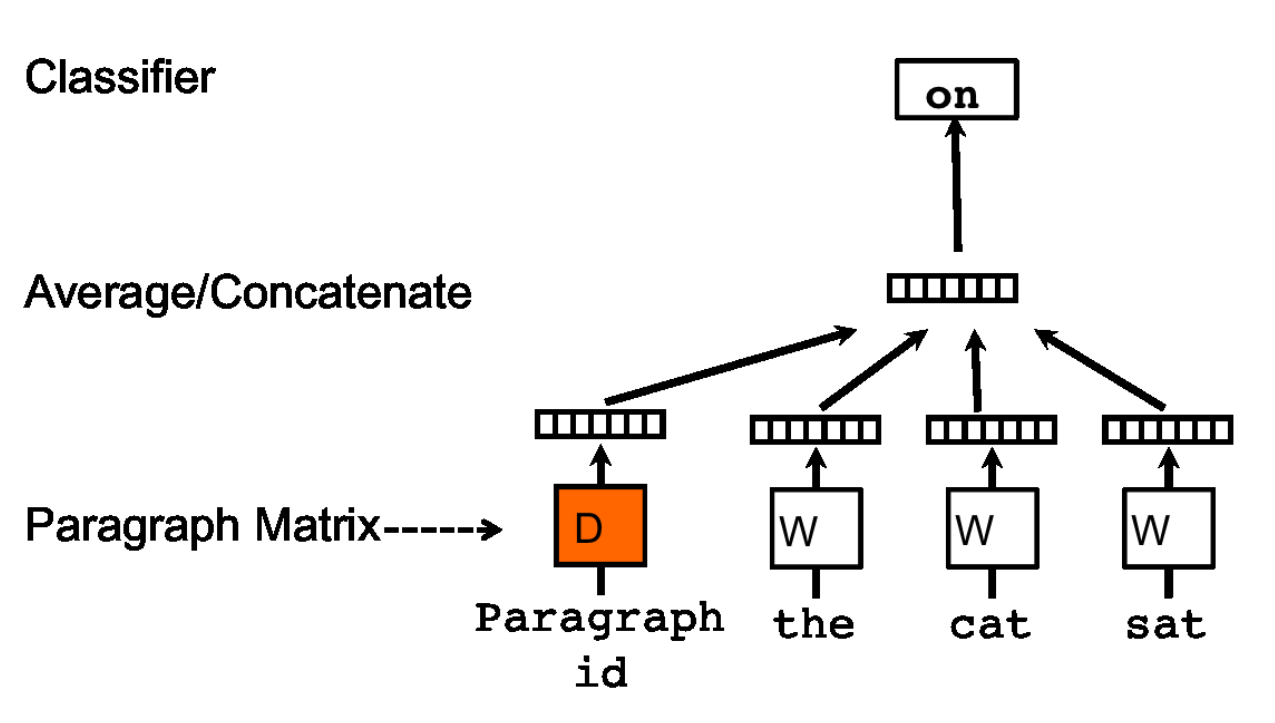
\includegraphics[width=250px]{../chapters/implementation/pics/doc2vec}
	\caption{\label{pic:doc2vec} Visualization of a training step of a Doc2Vec network {\cite{wuWordMoverEmbedding2018}}}
\end{figure}

\subsection{Selection of a document embedding technique}

Summarizing the previously discussed methods by three of their main characteristics - number of hyperparameters, maximum processable document length and type of model results in  \autoref{tab:overview_doc_embedding}.
\begin{table}
	\centering
	\begin{tabular}{ c | c | c }
		\hline 
		Technique & Max. document length & Type \\ \hline
		Tf-Idf BOW & unlimited & Probabilistic \\ \hline
		Latent Dirichlet Allocation & unlimited & Probabilistic \\ \hline
		Doc2Vec & unlimited & NN \\ \hline
		Word mover's embedding & unlimited & Kernel method \\ \hline
		BERT & 512 characters & NN \\ \hline
	\end{tabular}
	\caption{\label{tab:overview_doc_embedding} Table summarizing the key features of different document embedding techniques}
\end{table}

The model is now selected by exclusion. Since our database contains documents which are longer than 512 tokens and each token has a length of at least 1 character, BERT is eliminated as a potential document embedding technique. It would be possible to take word embeddings from BERT and average them in order to get a document embedding as it was proposed and further developed in \cite{deboomRepresentationLearningVery2016} for Word2Vec embeddings, but there was no scientific or non-scientific literature that suggested that this works for the case of contextualized BERT embeddings.
Furthermore the previous literature mapping study showed that there is not a lot of work done for explaining probabilistic models or models utilizing kernel tricks, therefore TF-Idf BOW, the LDA and the Word Mover's embedding are not of interest in this case. Only Doc2Vec remains, supporting both an unlimited document length and being of type 'NN' and therefore potentially being able to support at least 7 explainability techniques sourced from the mapping study and since neural networks are a focus for interpretability research at the moment, as visible in \autoref{fig:applicability_gamut}, even more techniques which are going to be developed in the future.

\section{Topic extraction}

Currently the only used topic extraction method is the LSA. Since the underlying SVD is a purely linear technique, the questions stands if the results of the topic extraction improve when nonlinear features are taken into account. One technique to perform an nonlinear, unsupervised dimensionality reduction is the \textit{Autoencoder}. This type of neural network consists of an encoder network and a decoder network as seen in \autoref{pic:autoencoder}. The encoder maps an input to an intermediate layer, while the decoder maps a vector from its representation in the intermediate layer to a vector in the vector space of the original input.

The composition of encoder and decoder is then trained to reconstruct the input from its intermediate layer via a standard backpropagation algorithm. Choosing the intermediate layer of lesser dimensionality compresses the input vectors, which constitutes as a dimensionality reduction. As Wang et al. \cite{wangAutoencoderBasedDimensionality2016} pointed out, an autoencoder can emulate the results of a PCA/SVD by choosing a linear activation function for all neurons and may even outperform it for other nonlinear activation functions.

Adding a sparsity constraint to the encoding network can help to describe a project by as little features as possible. Since the features could be interpreted as topics, this constraint helps the clustering task downstream.

\begin{figure}[t]
	\centering
	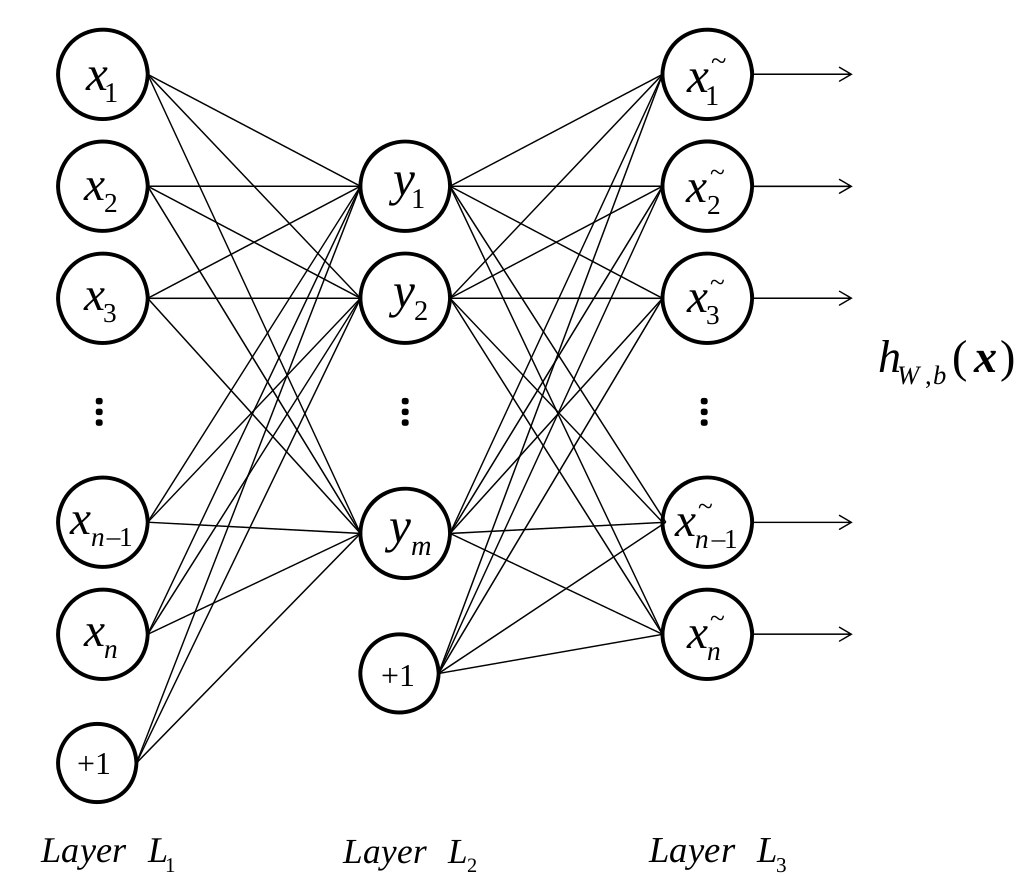
\includegraphics[width=250px]{../chapters/implementation/pics/autoencoder}
	\caption{\label{pic:autoencoder} Strucuture of a simple autoencoder {\cite{wangAutoencoderBasedDimensionality2016}}}
\end{figure} 

Training the model with an embedding dimension of 50, binary crossentropy as a loss function and Adadelta optimizer shows that the model achieves a loss of 0.005 after 75 epochs on the training set and approximately 0.01 on the validation set \autoref{pic:autoencoder_loss}.

\begin{figure}[t]
	\centering
	\includegraphics[width=400px]{/home/tim/HCC/IKON-backend/src/topicextraction/nlp/plots/autoencoder_loss}
	\caption{\label{pic:autoencoder_loss} Graph showing the training and validation loss of the autoencoder over progressing epochs}
\end{figure}

 

\section{Clustering}

As described in the beginning of this chapter a K-Means clustering would now classify the documents in the latent topic space. A problem that this approach poses is that the assumption that the Euclidian distance (EuD), which is the inert similarity measure of the K-Means algorithm \tk{Cite!} is meaningful in our vector space may not be true. \tk{Cite?} Another distance measure which may may encode more semantic meaning could be the previously mentioned \textit{Word Mover's Distance}. Since it uses the generated word embeddings and their order in the document to compute distances, it may be more suited for comparing texts and subsequently also yield better results for the clustering. This weighs even heavier if the corpus is vectorized as a sparse matrix since the Euclidian distance, as described in \autoref{chap:introduction}, looses its meaning . In our case, having embeddings from a Doc2Vec model, we don't have to deal with this additional problem, but the question remains if the two distance measures differ on our dataset.  
Comparing the distances between documents generated by both the Word Mover's distance and the Euclidian distance in \autoref{pic:wmd_eud_boxplot} it is apparent that there is indeed a difference. Therefore it is worth investigating if using this information improves the clustering results. 

\begin{figure}[t]
	\centering
	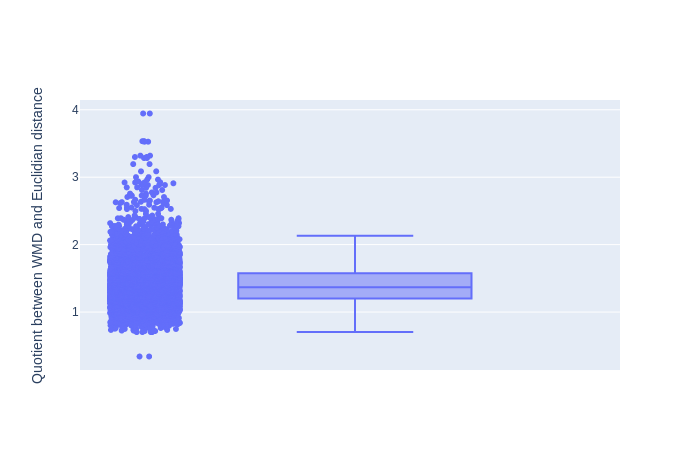
\includegraphics[width=400px]{/home/tim/HCC/IKON-backend/src/topicextraction/nlp/plots/wmd-eud}
	\caption{\label{pic:wmd_eud_boxplot} Boxplot showing the distribution of the quotients between WMD and EuD for all documents}
\end{figure}

Inspired by Liu et al. \cite{Liu:2018:INE:3219819.3220001} I chose a hierarchical clustering approach, specifically \textit{Agglomerative Clustering}, as a contending method to the K-Means algorithm. This method works bottom-up since in the beginning it considers every data point to be its own cluster. Now in every step two clusters are merged which minimize a given linkage metric. The distance calculations between points are performed by a lookup in a precomputed distance matrix which enables the usage of any given distance metric. Doing this until only one cluster remains, creates a binary tree, which describes the hierarchy of the data given the used metric. 

\section{Visualization}

In order to visualize all the results from the topic modeling pipeline I developed a D3.js-based interface, which is embedded in the Jupyter notebook in which the code for all the numerical computations resides. Since Jupyter is embracing the browser as a frontend, there is the possibility to embed arbitrary Javascript code in a cell and inject any kind of visualization. In order to do that I construct a JSON object containing all the results from the topic pipeline (vectorized documents as scatter points and linearized points, top words, the interpolated topography, model parameters etc.) and pass it into the Javascript code via Jupyter's $Javascript$ function and string interpolation which renders it in the browser.

The interface consist of a discrete slider controlling the granularity of the clustering, which translates to the number of clusters which are computed in the topic modeling pipeline. Furthermore there is a dropdown selection where one can switch between the scatter and the linearized variants of the scatter plots.
Beneath the parts of the interface which are connected to parameter selection, the top words for all clusters are displayed and even further down the plot is located in which each project is visualized as a circle. Changing any of these parameters result in an immediate change of the computed plot and the top words. Additionally one can hover over projects in order to reveal additional metadata about the project (project ID, title, top words).

\begin{figure}[t]
	\centering
	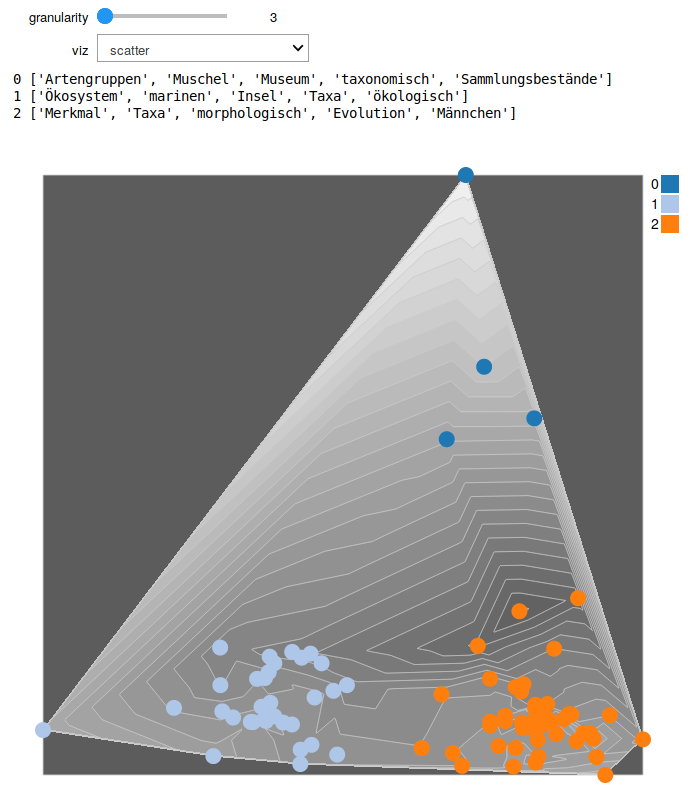
\includegraphics[width=300px]{../chapters/implementation/pics/interface}
	\caption{\label{pic:interface} Screenshot showing the exemplary interface}
\end{figure}

\section{Explainability techniques}

\subsection{Explainability technique: Linearization}

As Lipton \cite{liptonMythosModelInterpretability2016a} pointed out, a visualization is already an explainability technique in itself. Therefore we can use the vast amount of interaction design research to optimize the existing interface. 

One of the main problems of scatter graphs is overdrawing, also called clutter. This problem occurs when glyphs are close enough in a scatter plot so that they overlap each other. The higher the density of a region is, the harder it gets to perceive the total number of points and the harder it is to annotate the glyphs with additional data \cite{mayorgaSplatterplotsOvercomingOverdraw2013}. 

Normally this problem is hard to solve since the position of points in respect to each other encodes important information. Considering that in this case a high dimensional space is reduced to 2D, there are inherent reduction errors introduced into the distances between points and the absolute distances in 2D loose part of their semantic importance. Therefore it is possible to assume that instead of distances, the neighborhood of a point is more important, which leads to the possibility to map the scatter graph on a more regularized structure while preserving the neighborhood of points as well as possible. One way to do so, is to map the points in 2D onto a grid. This problem reduces to a linear assignment problem (LAP), where each point should be assigned to its nearest point in the grid while minimizing the global displacement error. A popular algorithm for that is the Jonker-Volgenant algorithm \cite{jonkerShortestAugmentingPath1987}. Jonker and Volgenant rephrase the LAP as a shortest path problem and by using augmenting paths improve the previously popular Hungarian algorithm to cubic worst-case complexity. As we will see in one of the next subsections, this technique also synergizes well with the cluster topography method, because the interpolation also get linearized and the topography gets expanded making it easier to see differences in the relief.

\subsection{Explainability technique: Top words}

Looking at \autoref{fig:pipelinestep_gamut} shows that local instance explanations as a strategy to explain the output of an unsupervised embedding algorithm are most prevalent among all sourced publications. Factoring in the two questions from \autoref{tab:overview_viz_questions} which deal with the most prominent topics and the similarity between projects and clusters I will rank the input features to the document embedding and topic extraction step for each document and cluster. 

Assume that a document is described as a vector $c \in \mathbb{R}^k$ in the latent topic space. In order to show the most important features in the document there are two possible ways. The first option factors in how well the topic extraction projects the documents. Taking the vector in the latent space, firstly the inverse dimensionality reduction is applied in order to transform the vector into the embedding space. Both the LSA and the autodecoder approach have this opportunity, but they differ greatly in quality of this reconstruction. Since the LSA is a linear method, the back projection yields all documents on a hyperplane, while the autodecoder is able to minimize the reconstruction loss through its inherent nonlinearity. 
The second option disregards the capabilities of the topic extraction model to reconstruct a vector in the embedding space from a vector in the latent topic space. Instead for projects the embedding vector is taken directly or for cluster centers the average from all assigned projects in the embedding space is calculated as a representative. For the sake of implementational simplicity the second option was used for this thesis despite its shortcomings.

Now that the document vector is in its embedding space we will make use of a special ability of the Doc2Vec model. As described in the previous section the model does not only train document vectors, but it also generates word embeddings in the same space. The revolution the Word2Vec model, as a base of the Doc2Vec model, presented was that the generated embeddings and their relations to each other encoded semantic relations. Although there is no literature on this, it is a hypothesis that this behaviour also applies to the embedding of document and word vectors into one space. This leads to the possibility of describing a document by its nearest word vectors. An exemplary analysis shows that there seems to be a valid semantic structure in the relations between tokens and between tokens and documents. As a German native speaker it is easy for me to verify that the word queries in \autoref{tab:semantic_connectivity_words} are indeed semantically well connected. The results of the document queries in \autoref{tab:semantic_connectivity_docs} on the other hand are hard to verify since most documents are very specific, scientific texts. I picked two projects and their top words which I was able to understand without relying on external information. The first three top words are indeed well connected to the topic of the corresponding project, but the last two ones seem to be off. This exemplary analysis speaks in favor of the hypothesis that there are indeed semantic connections document vectors and word vectors.

\begin{table}
	\centering
	\begin{tabular}{ p{6cm} | p{6cm} }
		"Evolution" & "Diversität" \\ \hline
		\begin{enumerate}
			\item evolutionären
			\item evolutionäre
			\item evolutionärer
			\item phylogenetische
			\item Artbildung
		\end{enumerate} & 
		\begin{enumerate}
			\item Artenzusammensetzung
			\item Biodiversität
			\item Taxa
			\item taxonomisch
			\item Lebensräumen
		\end{enumerate} \\
	\end{tabular}
	\caption{\label{tab:semantic_connectivity_words} Table showing the top five similar words for two queries by word}
\end{table}

\begin{table}
	\centering
	\begin{tabular}{ p{6cm} | p{6cm} }
		\href{https://gepris.dfg.de/gepris/projekt/387798678}{'Ambitionierte Amateure' - Europäische Filmclubs in den langen 1960er Jahren} & \href{https://gepris.dfg.de/gepris/projekt/160874660}{Netzwerke im europäischen Handel des Mittelalters} \\ \hline
		\begin{enumerate}
			\item Kulturpraxis
			\item Kulturzentren
			\item alltagsweltlich
			\item pain
			\item Ceuta
		\end{enumerate} & 
		\begin{enumerate}
			\item Opportunitätskosten
			\item Diskursteilnehmer
			\item evoluieren
			\item schloss
			\item Staphylococcen
		\end{enumerate} \\
	\end{tabular}
	\caption{\label{tab:semantic_connectivity_docs} Table showing the top five similar words for two queries by document}
\end{table}

Extracting top words for the existing TfIdf method is simpler, because the every entry in the embedding vector has a one-to-one correspondence to words. Taking the biggest n entries yields n top words due to the TfIdf measure directly being a indicator for the amount of contained information and subsequently importance.

\subsection{Explainability technique: Cluster topography }

The hypothesis on which this technique is grounded is that clusters in a high dimensional space are inherently hard to interpret, because the cluster does not exist as an explicit object. A cluster is rather an abstract concept and solely consists of the points which are connected to it via a membership assignment. Especially once the points which form a cluster get reduced into a 2D or 3D space distances get distorted, a problem that was discussed in a previous subsection. Information on the position and form of the clusters is not easily obtainable anymore. One way to mitigate this is to extract artifacts in the high dimensional space and carry it over into the 2D space where the points can be visualized.

Motivated by the explanatory nature of the interaction which the non-technical experts will carry out, the quality of each point fitting into its cluster could be an interesting pointer to make potentially contrastive deductions concerning the structure of the clusters.

This technique computes an uncertainty measure for each point which describes how well it fits into its assigned cluster. A straightforward idea would be to assign each point the Euclidean distance between the point and its cluster centroid. Small distances speak in favor of the hypothesis that a point fits well into its cluster, while bigger distances speak in favor of the contrary. After the projection into 2D a topography is interpolated with the points and their Euclidean distances as fulcrums. This intendedly invokes the notion of a geographical surface since this most sciences, especially at a natural history museum, work often with such kind of maps. Making sure that the peaks of this topography corresponds to points which fit very well into their clusters enlarges the metaphor and ensures that people are intuitively able to understand the visualization. 

The problem with this approach is that, firstly the Euclidean distance may not be well suited for such vector spaces, as discussed earlier, and points in different clusters cannot be compared since volume-wise larger clusters exhibit a higher distance for each point than ones which are more compact, albeit having a similar fitness in relation to the points of the same cluster. Secondly points may exhibit the same fitness and lie close together in 2D, but may be on two opposing ends of an n-dimensional sphere in the latent space. 

The second problem is harder to tackle since that is one of the inherent problems of dimensionality reductions and therefore I will present an argument for an alternative similarity measure.

The main information that this technique should convey is how well the clustering method captured the structure of the high dimensional space which can be expressed by measuring how sure the method is about the cluster assignment for each point. One measure capturing this information is the silhouette score \cite{rousseeuwSilhouettesGraphicalAid1987}. The silhouette score takes, for each sample, also the nearest, non-assigned cluster into account, computes the mean intra-cluster distance $a$ and the mean nearest-cluster distance $b$ and scores them as $\frac{(b-a)}{\max{a,b}}$. This leads to a score between -1 and 1, where a negative value denotes that the point was assigned to the wrong cluster since the nearest, not-assigned one is closer than the assigned cluster. The normalization of this score makes it possible to compare the fitness of points between clusters as well. 

I developed this technique in cooperation with Christoph Kinkeldey and Jesse Josua Benjamin, presented it at TrustVis19 in Porto, Portugal, as well as published it in \cite{christophkinkeldeySupportingInterpretabilityClustering2019}.


\section{Model selection using topic coherence}

Now that there is an option to choose between two options for the embedding, topic extraction and classification step of the generic topic modeling pipeline, it is interesting to see which combination of these methods performs the best. A popular method to measure the quality of a topic modeling pipeline is the Coherence Score. Röder et al.\cite{roderExploringSpaceTopic2015a} proposed an agnostic way to evaluate topic models, unifying several contending methods at that time. Their generic pipeline consists of four steps: segmentation, probability calculation, confirmation measure and aggregation. The segmentation step consists of segmenting the dictionary, the set of all occuring words, into subsets. Then for every word a probability is calculated using a reference corpus, which is used in the subsequent step where a confirmation measure scores the word pairs concerning how often they appear together in documents or in sliding windows over documents. A last step aggregates all the agreement scores and calculates an overall coherence score for the segmentation on the supplied reference corpus. In our case the segmentation is done by supplying the top words for all clusters.  In this analysis the $c_v$ measure was chosen, because it displayed the highest correlation (0.731) with human ratings in the experiments of Röder et. al.

Plotting the coherence scores over different embedding, topic extraction and clustering models and different number of clusters reveals (\autoref{pic:tm_quality}) , surprisingly, that the combination with the best scores is an TfIdf embedding, an LSA topic extraction, followed by an Agglomerative Clustering with 10 clusters. The combination of TfIdf embeddings and an autoencoder couldn't be tested since in order to feed sparse matrices to a Keras neural network there is a considerable amount of work involved. In order to keep this thesis reasonable, this analysis is considered in the Outlook.

\begin{figure}[t]
	\centering
	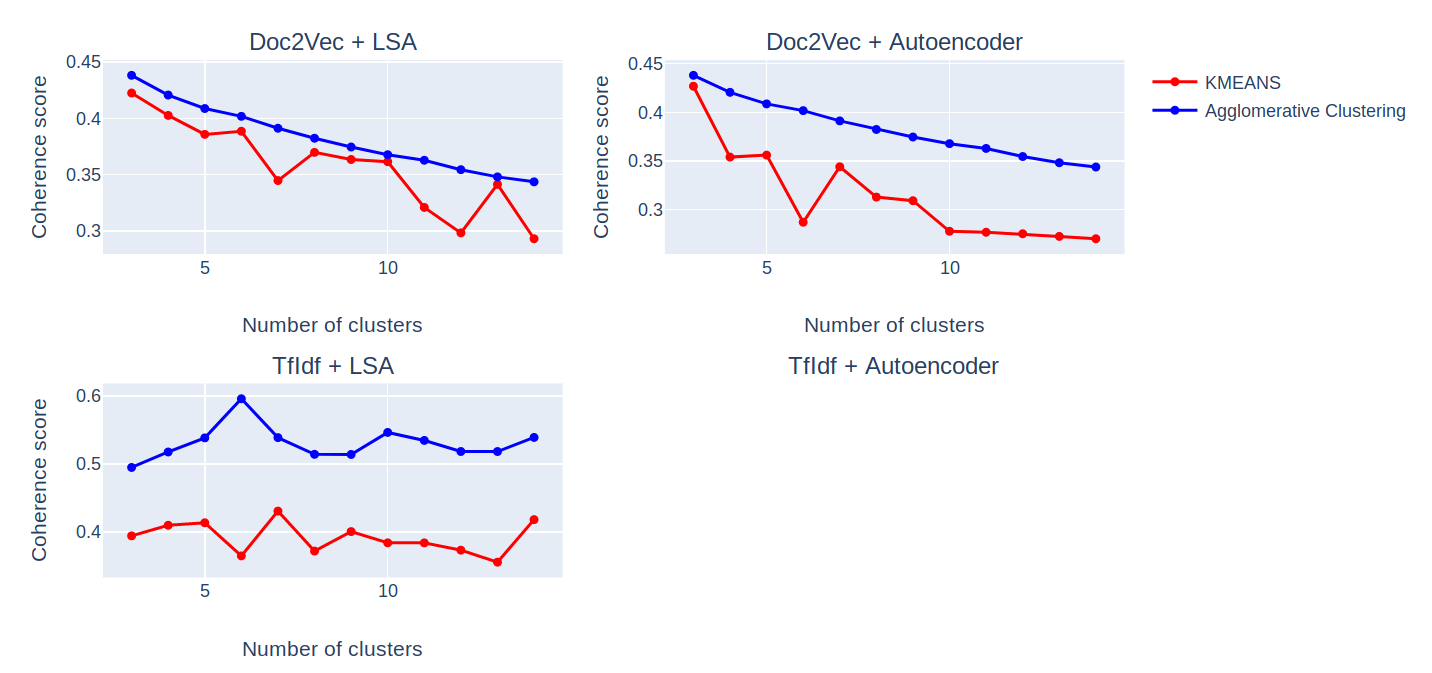
\includegraphics[width=400px]{/home/tim/HCC/IKON-backend/src/topicextraction/nlp/plots/tm_quality}
	\caption{\label{pic:tm_quality} Graph showing the quality of the topic modeling while varying the embedding, topic extraction and clustering model}
\end{figure}

Plotting this combination of models and parameters in \autoref{pic:best_coherence_plot} reveals that there is one huge cluster (cluster 0) while the other 9 clusters contain maximally five projects. A further analysis of the dominating cluster also showed that although its top words suggest projects connected to evolution and biology, there are also a number of projects which deal with geology and paleontology. Interestingly, perturbating the parameters of all models does not change the fact that such a huge cluster forms speaking in favor of the hypothesis that these projects indeed form a huge cluster in the high embedding space.

\begin{figure}[t]
	\centering
	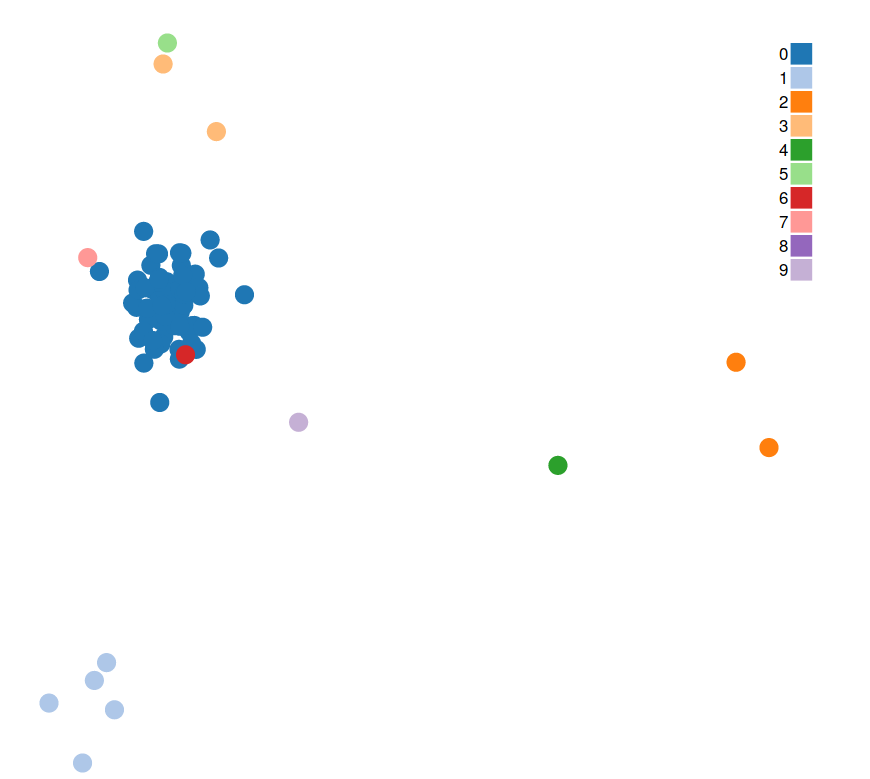
\includegraphics[width=400px]{../chapters/implementation/pics/best_coherence_plot}
	\caption{\label{pic:best_coherence_plot} Plot for the parameter and models with the best coherence score}
\end{figure}

\begin{table}
	\centering
	\begin{tabular}{c | c}
		0 & Datum, Evolution, morphologisch, Taxa, ökologisch \\ \hline
		1 & Sackflügelfledermaus, Abwanderungsverhalten, Weibchen, Männchen, Harem \\ \hline
		2 & Western, Mountains, Kaokoveld, Fauna, Escarpment \\ \hline
		3 & Tansania, biostratigraphische, palynologisch, Tendaguru, Palynologie \\ \hline
		4 & Acentropinae, Philippinen, Trichoptera, Lepidoptera, Reliktendemiten \\ \hline
		5 & SCHRANK, gesichert, Flora, Sauropoden, Gymnospermen \\ \hline
		6 & Praktik, kolonisieren, Mediziner, Gesundheitsbehörden, Malaria \\ \hline
		7 & Magmaozeans, Magmaozean, Planetare, Impaktprozess, Impaktors \\ \hline
		8 & Kurzexpedition, Basilosauridae, Pabdeh, Ablagerungen, Iran \\ \hline
		9 & Hauptexporteur, Kieselalgendiversität, Känozoikum, Silikatverwitterung, Kieselalgen \\ \hline
	\end{tabular}
	\caption{\label{tab:best_coherence_table} Table showing the top words for {\autoref{pic:best_coherence_plot}}}
\end{table}

At this point I gathered feedback from the researchers from project IKON and their answers suggested that problems may occur trying to visualize such dominating structures in scatter plots. \tk{Proper argument?}
Therefore I turned to the second best performing combination of models which is a TfIdf embedding, an LSA topic extraction and a K-Means clustering - which is effectively the topic modeling pipeline which was existing at the beginning of the thesis. Since all the implemented explainability technique also work for this combination of methods, I sticked with it for the validation. 
% ---------------------------------------------------
% ----- Conclusion of the template
% ----- for Bachelor-, Master thesis and class papers
% ---------------------------------------------------
%  Created by C. Müller-Birn on 2012-08-17, CC-BY-SA 3.0.
%  Freie Universität Berlin, Institute of Computer Science, Human Centered Computing. 
%
\chapter{Validation}
\label{chap:validation}

In order to show how the implemented explainability techniques may help a non-technical expert understanding the output generated by the pipeline, a proper user study would be needed. Since that is a task which would fill a bachelor thesis on its own, I resorted to a strategy which involves less work, but also delivers qualitative insights into the interaction between a user and the topic modeling pipeline and its visualization - the cognitive walkthrough. Performing this method involves seeing things from the perspective of a fictive user and interacting with the application in their stead.
Since the nature of this visualization supports exploratory interactions in the first place, standard approaches for cognitive walkthroughs, like they are formulated in \cite{whartonUsabilityInspectionMethods1994}, do not work well due to the necessity of coding an interaction sequence prior to the simulated interaction. Allendorf et al. \cite{allendoerferAdaptingCognitiveWalkthrough2005} adapted the well-established method of cognitive walkthroughs to this kind of use case. Their method consists of defining a persona, goals for the interaction and possible steps which can be taken in the visualization. With this setup an action is performed which seems most applicable to reach the current goal and afterwards the following four questions are answered:
\begin{enumerate}
	\item What effect was the user trying to achieve by selecting this action?
	\item How did the user know that this action was available?
	\item Did the selected action achieve the desired effect?
	\item When the action was selected, could the user determine how things were going?
\end{enumerate}

\section{Setup}
The fictive user is a postdoctoral researcher at the Museum für Naturkunde Berlin. His background is characterized by the following features:
\begin{itemize}
	\item \textbf{Education}
	Is a postdoctoral researcher of biology specializing in evolutionary theory
	
	\item \textbf{Relevant work experience}
	Currently working on a project called "Variabilität von MHC-Genen bei der Sackflügelfledermaus Saccopterix bilineata" investing the genetic variability of bats
	
	\item \textbf{Experience with user interface design and usability assessment}
	Has no prior knowledge of interface design or usability assessment
	
	\item \textbf{Operating systems and software packages used frequently}
	Microsoft Windows; Microsoft Office (Word, Excel, PowerPoint); Microsoft Outlook; Mozilla Firefox; Microsoft Media Player; LaTeX; Zotero
\end{itemize}

As described in the Introduction, there are no common meeting rooms for the scientific staff at the museum. The interface is therefore positioned on a location which has the biggest throughput in the museum - in this case the side entrance which is exclusively used by the museum's staff.
The scenario and the context for this exemplary interaction is as follows:

	 One day after work, the fictive user is coming down the wide stairway of the side building he works in and sees once more the display with the visualization he passes every day on his way to and from work. This time the curiosity is stronger than the urge to go home and since he already heard that the museum financed a huge initiative to foster intra-organizational, scientific exchange, he decides to see what that application has to offer.


Looking at the questions formulated in the beginning of this thesis, we can now derive specific tasks this user may want to complete to answer the questions:
\begin{enumerate}
	\item Identify dominating research areas
	\item Find his own project
	\item Explore the projects in the same cluster
	\item Explore the projects in the vicinity of his own cluster
\end{enumerate}

The prototypical interface provides the following actions in order to manipulate the visualization:
\begin{enumerate}
	\item Investigate metadata for a project (title, ID and top words)
	\item Investigate top words for all clusters
	\item Change the number of clusters
	\item Switch between the linearized view and the scatter view
\end{enumerate}



\section{Cognitive Walkthrough} 

This cognitive walkthrough shows that the implemented explainability techniques help a non-technical expert to navigate in the visualization as well as understand why certain projects are located as they are since almost every step utilizes at least one of the techniques. Furthermore it unveiled a number of usability issues with the visualization. The first found problem is dismissable since the presented interface is not the final one which is going to go live, but the second may hinder the interaction with the visualization even in the actual prototype.

\newpage

\begin{longtable}[l]{| p{.4\textwidth} | p{.6\textwidth}  |} 
	\hline
	Description & Usability Impact \\ \hline \hline
	The label for the dropdown selection between the scatter plot and the linearized view does not properly describes what it does. & 
	Uncertainty about the usage of a tool may disturb a user in the inference task, therefore a descriptive name for this selection should be chosen. \\ \hline
	There is no visual connection between views while changing the cluster or view parameters. &
	Perturbing these parameters does not change the underlying displayed corpus, but the recomputation of the full pipeline may lead, due to the random initialization of the K-Means algorithm, to dramatically different outputs. Tracking these changes is quite hard and therefore after each change the user has to orient himself in the visualization anew. Adding animated transitions could help alleviating this problems by introducing object permanence in the views. \\ \hline
	
	
	\caption{Table summarizing the found usability design issues} 
	\label{tab:usability_problems}
\end{longtable}

% ---------------------------------------------------
% ----- Conclusion of the template
% ----- for Bachelor-, Master thesis and class papers
% ---------------------------------------------------
%  Created by C. Müller-Birn on 2012-08-17, CC-BY-SA 3.0.
%  Freie Universität Berlin, Institute of Computer Science, Human Centered Computing. 
%
\chapter{Conclusion}
\label{chap:conclusion}

As stated in the Introduction, this thesis was conducted in order to study what kind of explainability techniques for NLP exist and how they could support a non-technical expert in understanding the output from the system.

The first step was a systematic literature mapping study according to Petersen et al. \cite{petersenSystematicMappingStudies} which unveiled that I was able to confirm the findings of Lipton \cite{liptonMythosModelInterpretability2016a} and Miller \cite{millerExplanationArtificialIntelligence2017} in the domain of NLP.
Furthermore the results from the literature mapping study suggest that most of the current research focuses on supervised methods, such as neural networks, and these models are mainly made interpretable through local instance explanations. A proper definition of interpretability or an analysis of how a method influences interpretability lacks in a majority of publications on the other hand.

Based on these findings I was now able to take each component of the general topic extraction pipeline in \autoref{pic:general_topic_extraction_pipeline} and propose and implement a contending method. Each method was evaluated according to standard measures in order to ensure proper performance. Three out of four components where also augmented by explainability methods, while none of these techniques was implemented directly from one of the sourced papers, because none was able to answer the questions I formulated in the beginning and also .
Following an analysis investigating the interplay between all implemented methods, the decision was made to remain with the existing pipeline, but augment it by the proposed explainability techniques.

A cognitive walkthrough simulating a researcher doing an exploratory interaction unveiled a number of usability issues, but also showed how the implemented techniques support the user in making inferences about the output of the topic modeling pipeline.  

\section{Outlook}   
As discussed in \autoref{chap:literature_analysis} and visible in the results of the literature mapping study, there are a number of additional explanation strategies which could be applied to the augmented topic modeling pipeline.

Although the performance of Agglomerative Clustering didn't seem to satisfy the needs of the application, the idea of explaining a model by an induced taxonomy is still very interesting \cite{Liu:2018:INE:3219819.3220001}. Factoring in that the majority of the staff at the museum are trained biologists and taxonomies are widely used in this scientific discipline, these structures may be a very useful metaphor to present information to these non-technical experts.

Furthermore during the work on this thesis another potential question, additional to the ones defined in \autoref{tab:overview_viz_questions}, arose:
\begin{center}
	What kind of potential projects exist in the space between projects?
\end{center}
One of the already used techniques could be used to deliver potential answers . If the current LDA reduction gets replaced by a special kind of autoencoding, called variational autoencoding (VAE), it should be possible to generate meaningful vectors in the latent topic space and via the previously discussed methods also top words for these potential projects. 

Asides from additional explainability strategies and further model tuning, the whole system needs to be subjected to complete and rigorous user test with non-technical experts from the museum. The cognitive walkthrough included in this thesis does deliver a few insights into the usability of the application and the interaction with the topic modeling pipeline, but only a test in the situational context of the environment of the museum can convey reliable information concerning the interpretability of the used algorithms and the inferences the users are able to make using the system.


%---------------------------------------------------
%----- Appendix   
%---------------------------------------------------
\backmatter
% ---------------------------------------------------
% ----- Appendix of the template
% ----- for Bachelor-, Master thesis and class papers
% ---------------------------------------------------
%  Created by C. Müller-Birn on 2012-08-17, CC-BY-SA 3.0.
%  Freie Universität Berlin, Institute of Computer Science, Human Centered Computing. 
%

\chapter{Appendix}
\label{ch:Appendix}

\begin{figure}[t]
	\centering
	\includegraphics[angle=90,origin=c,width=330px]{/home/tim/HCC/IKON-backend/src/topicextraction/nlp/nlpflowchart_old}
	\caption{\label{pic:IKON_pipeline} BPMN process diagram of the existing topic modeling pipeline}
\end{figure}

\begin{figure}[t]
	\centering
	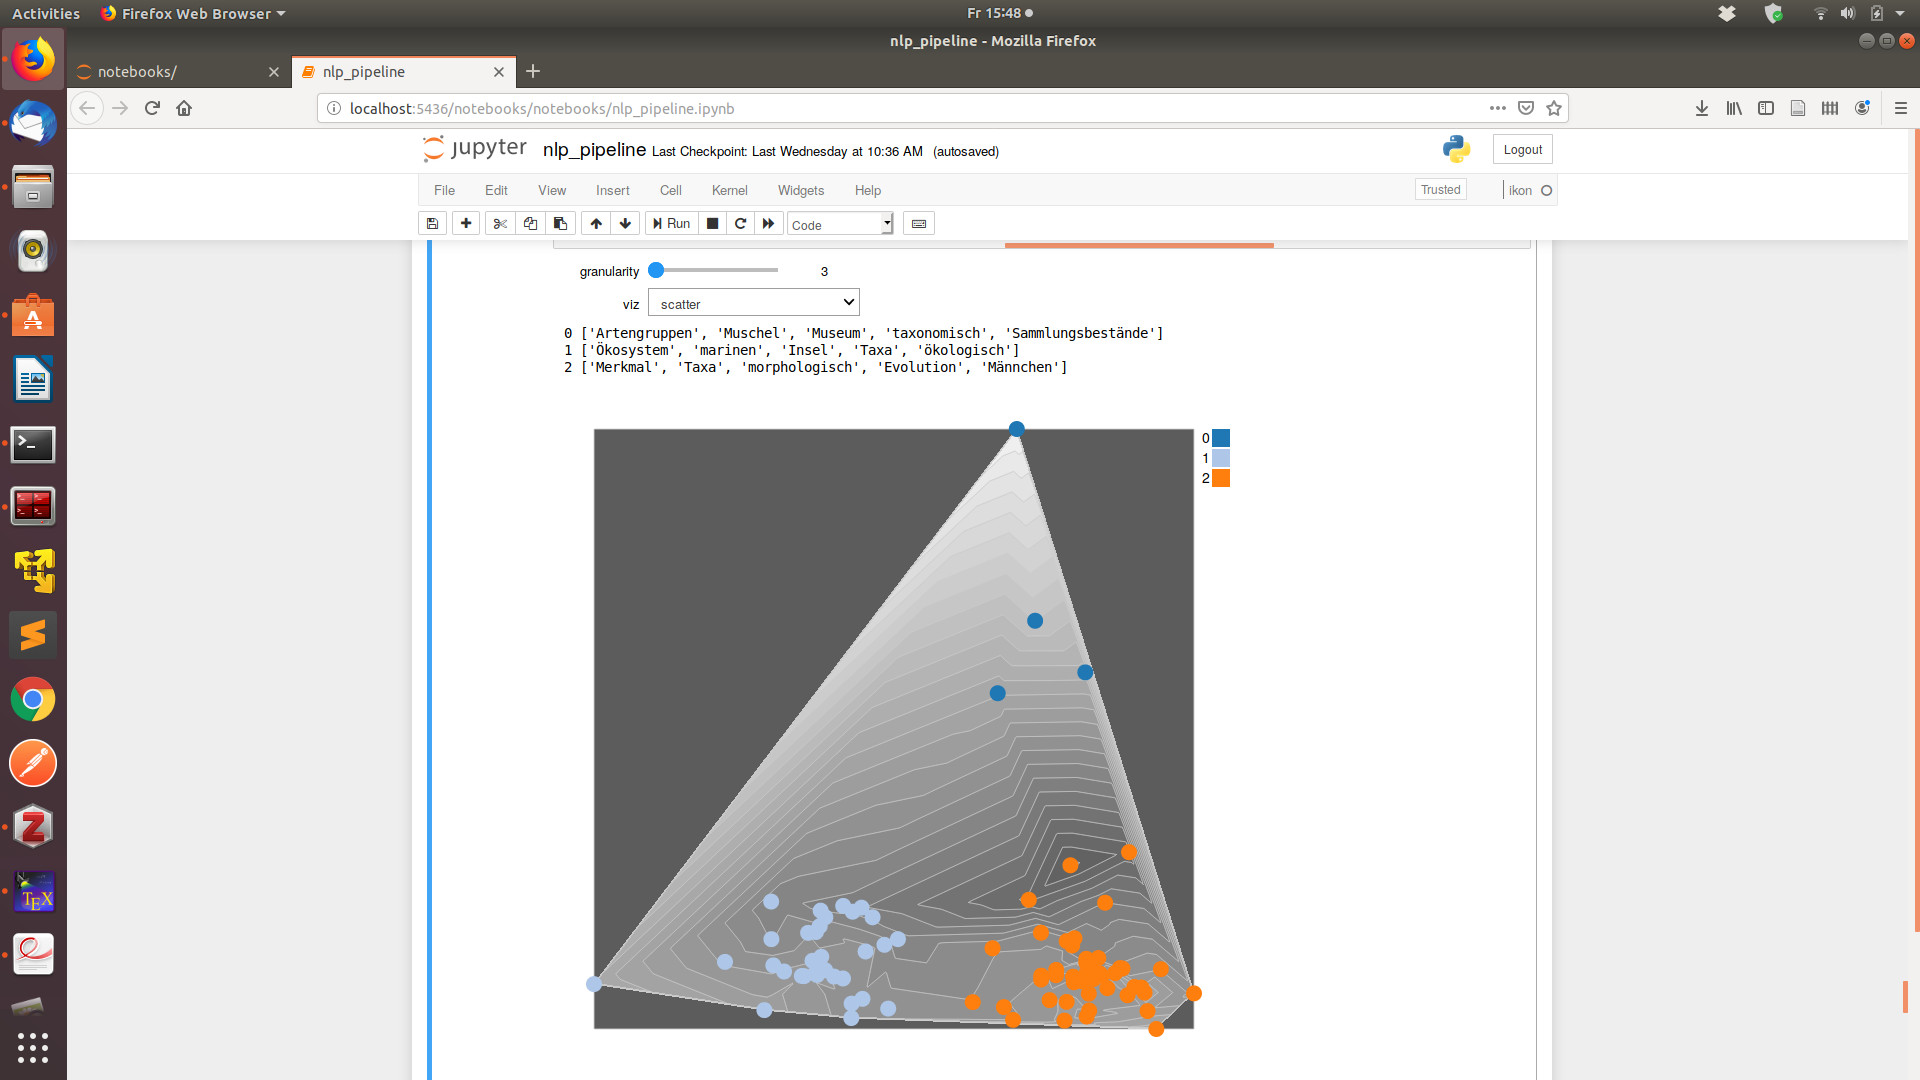
\includegraphics[width=400px]{../chapters/validation/pics/1}
	\caption{\label{pic:step1} Cognitive Walkthrough step 1}
\end{figure}

\begin{figure}[t]
	\centering
	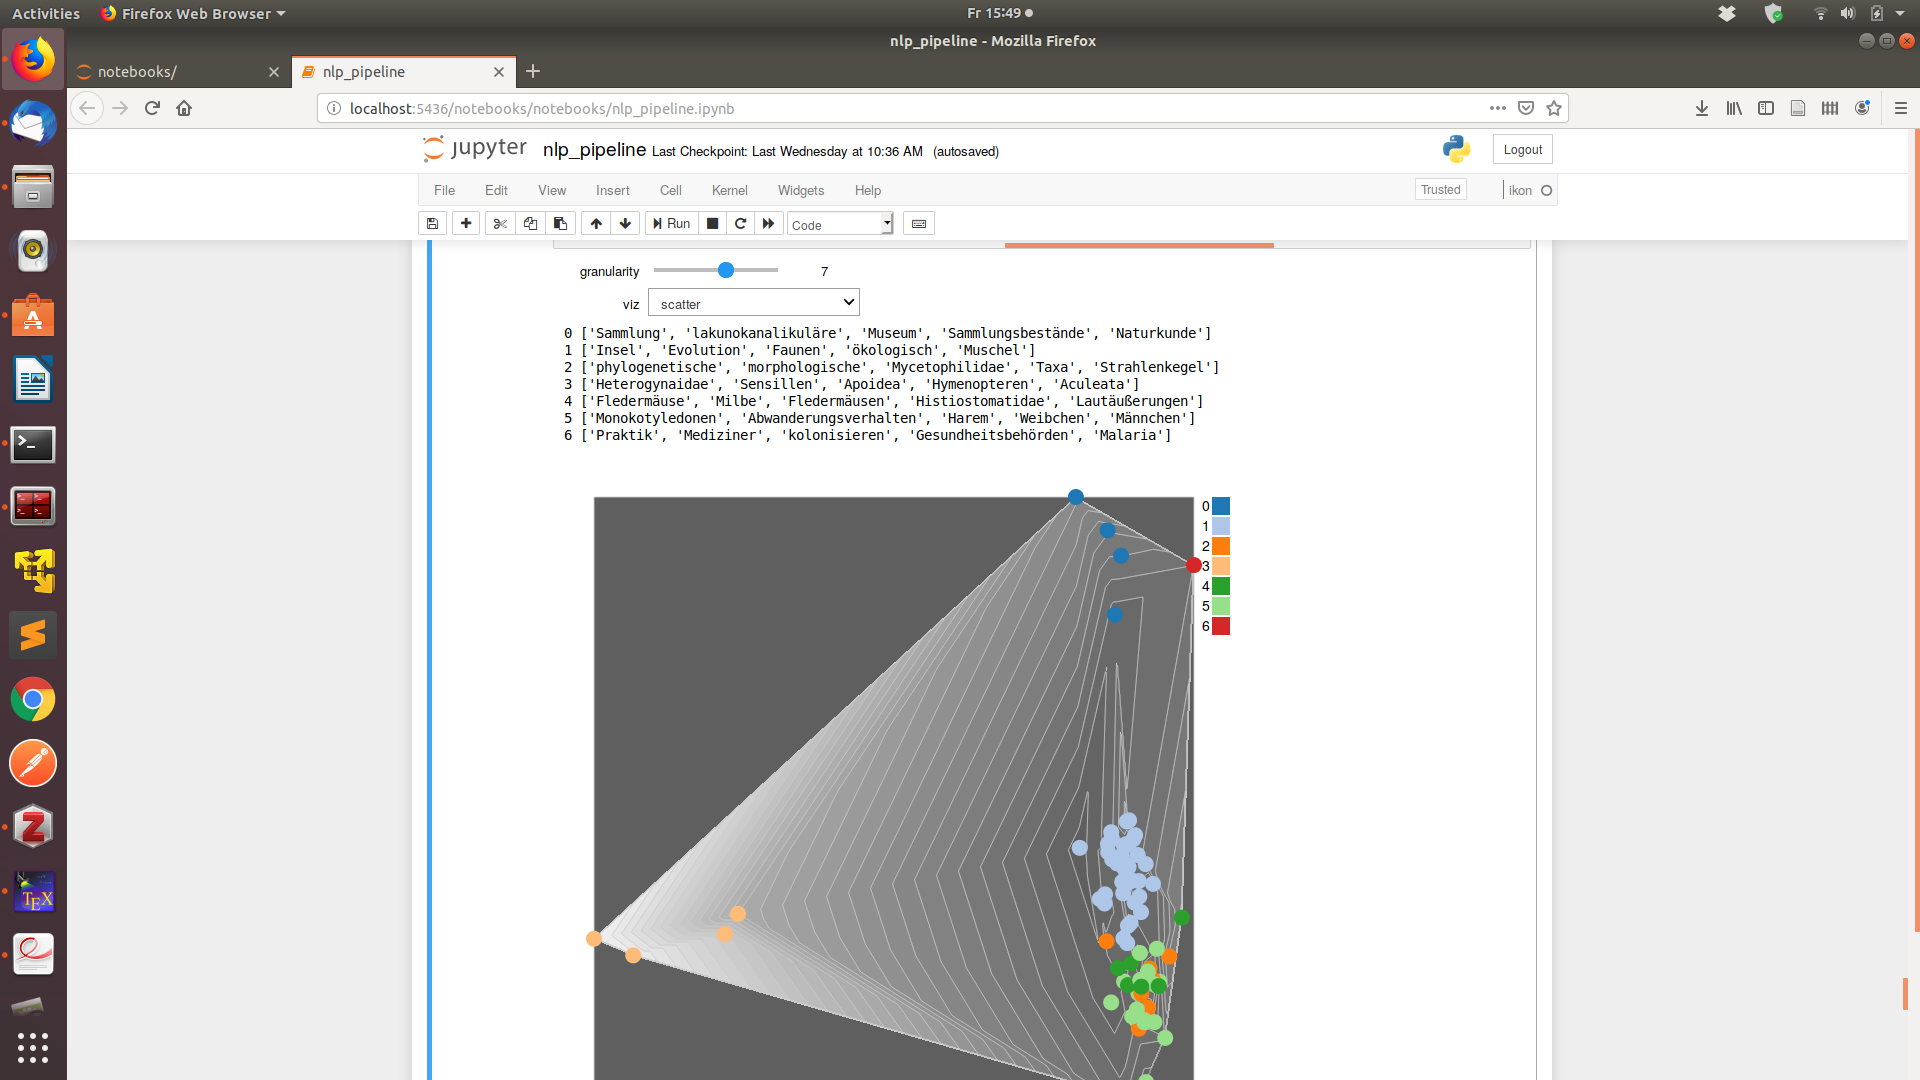
\includegraphics[width=400px]{../chapters/validation/pics/2}
	\caption{\label{pic:step2} Cognitive Walkthrough step 2}
\end{figure}

\begin{figure}[t]
	\centering
	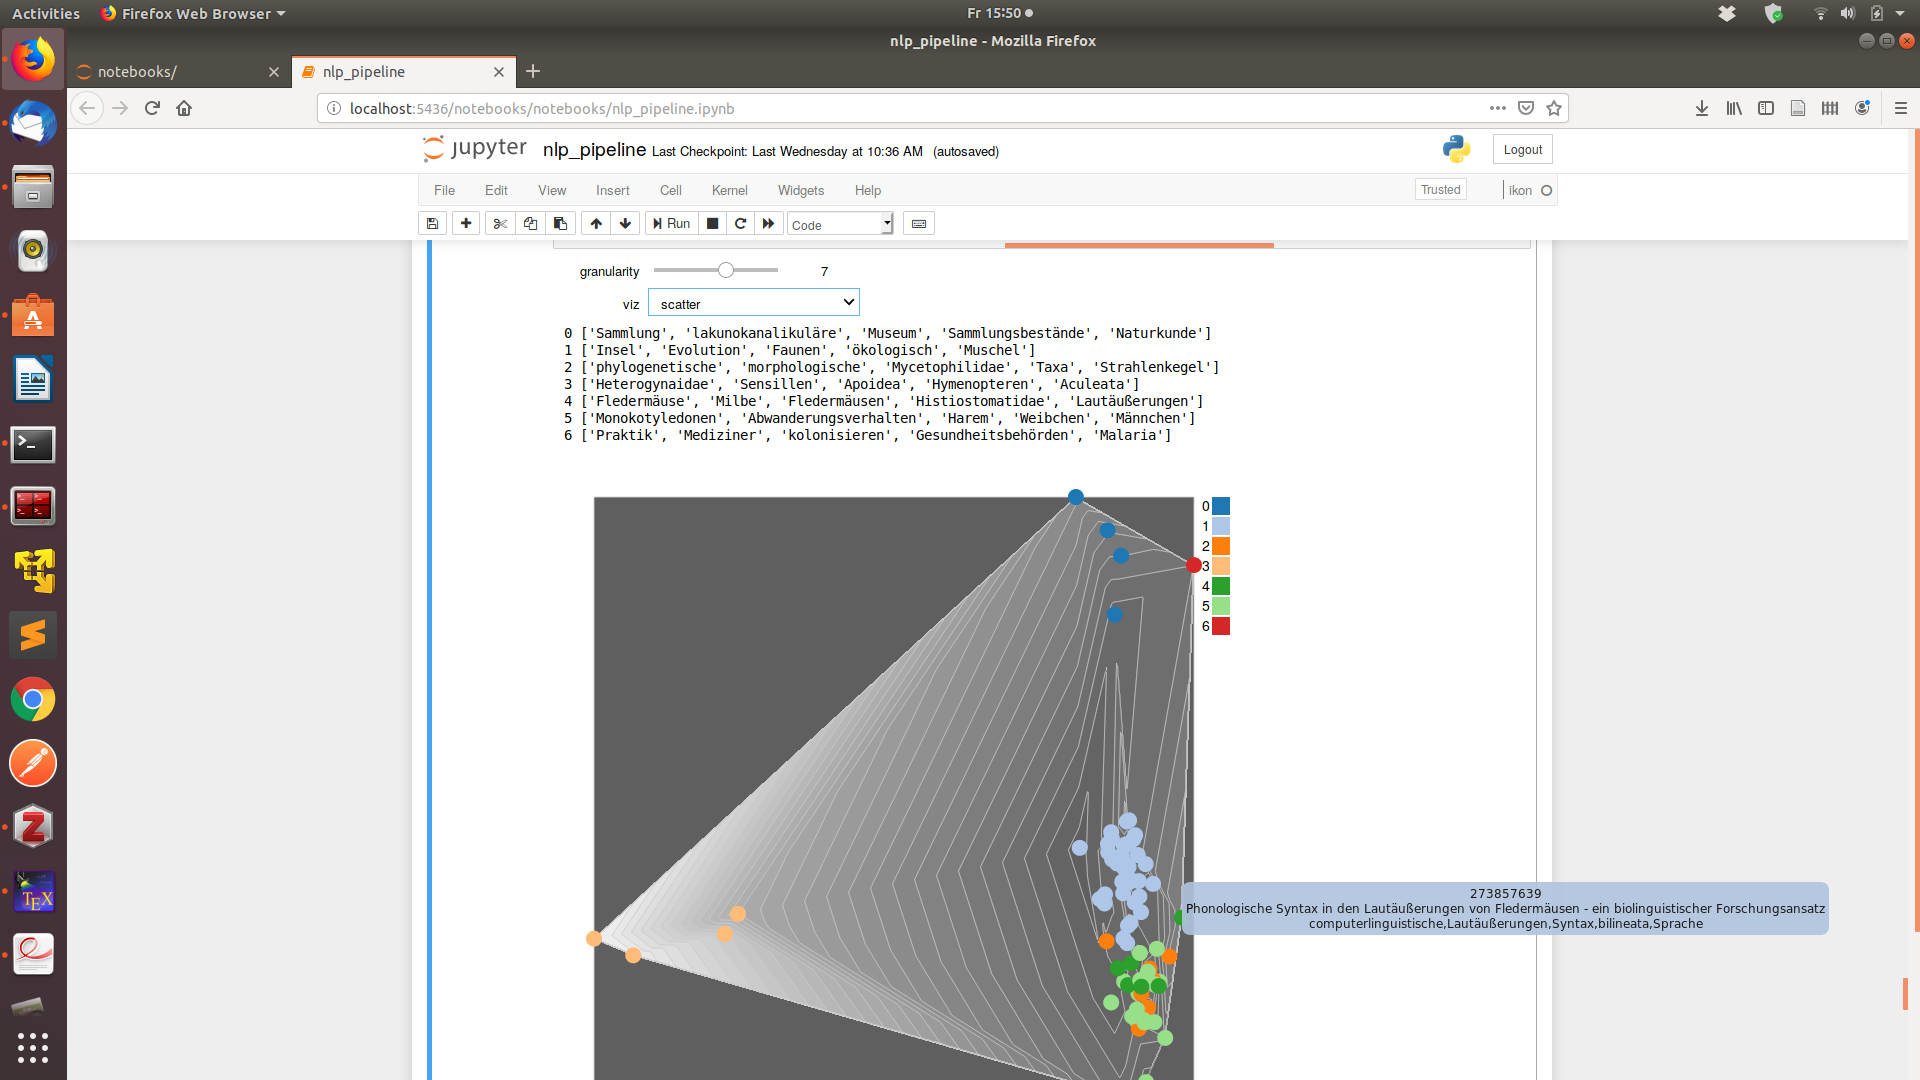
\includegraphics[width=400px]{../chapters/validation/pics/3}
	\caption{\label{pic:step3} Cognitive Walkthrough step 3}
\end{figure}

\begin{figure}[t]
	\centering
	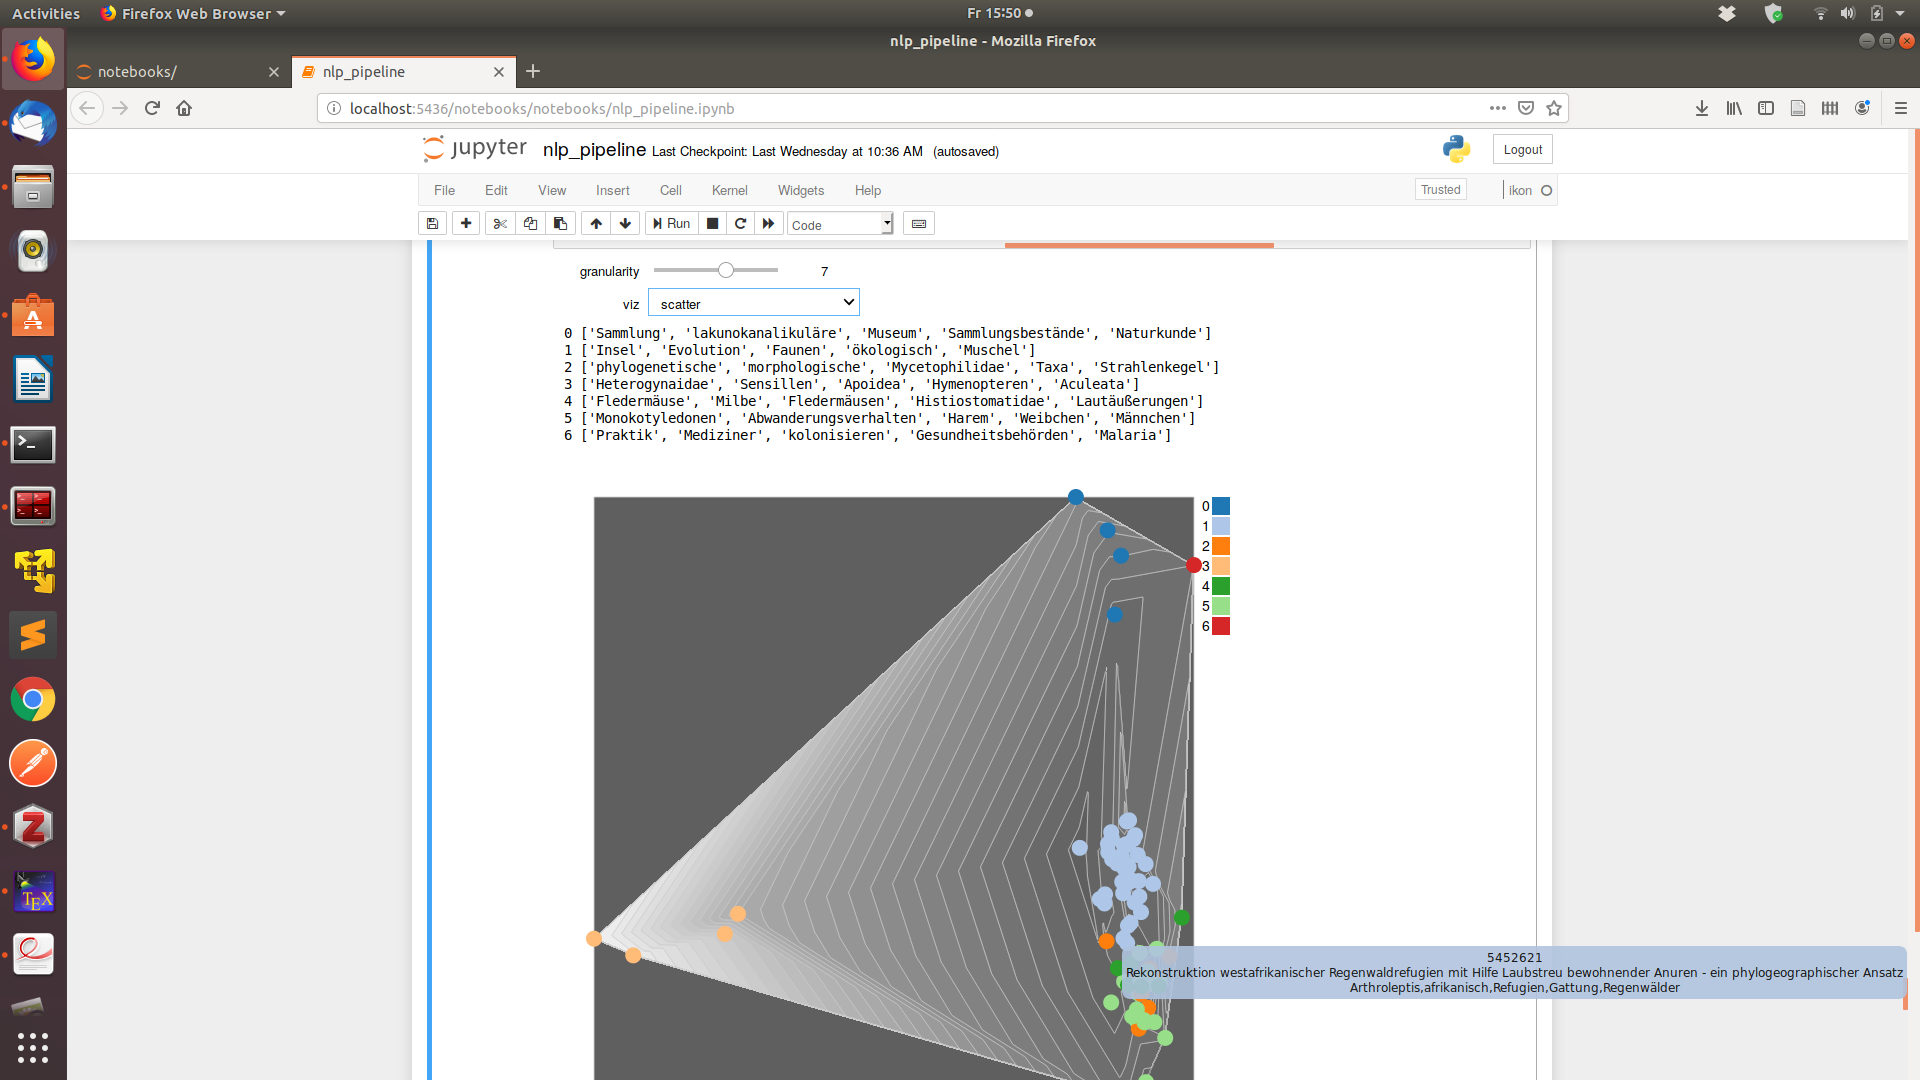
\includegraphics[width=400px]{../chapters/validation/pics/4}
	\caption{\label{pic:step4} Cognitive Walkthrough step 4}
\end{figure}

\begin{figure}[t]
	\centering
	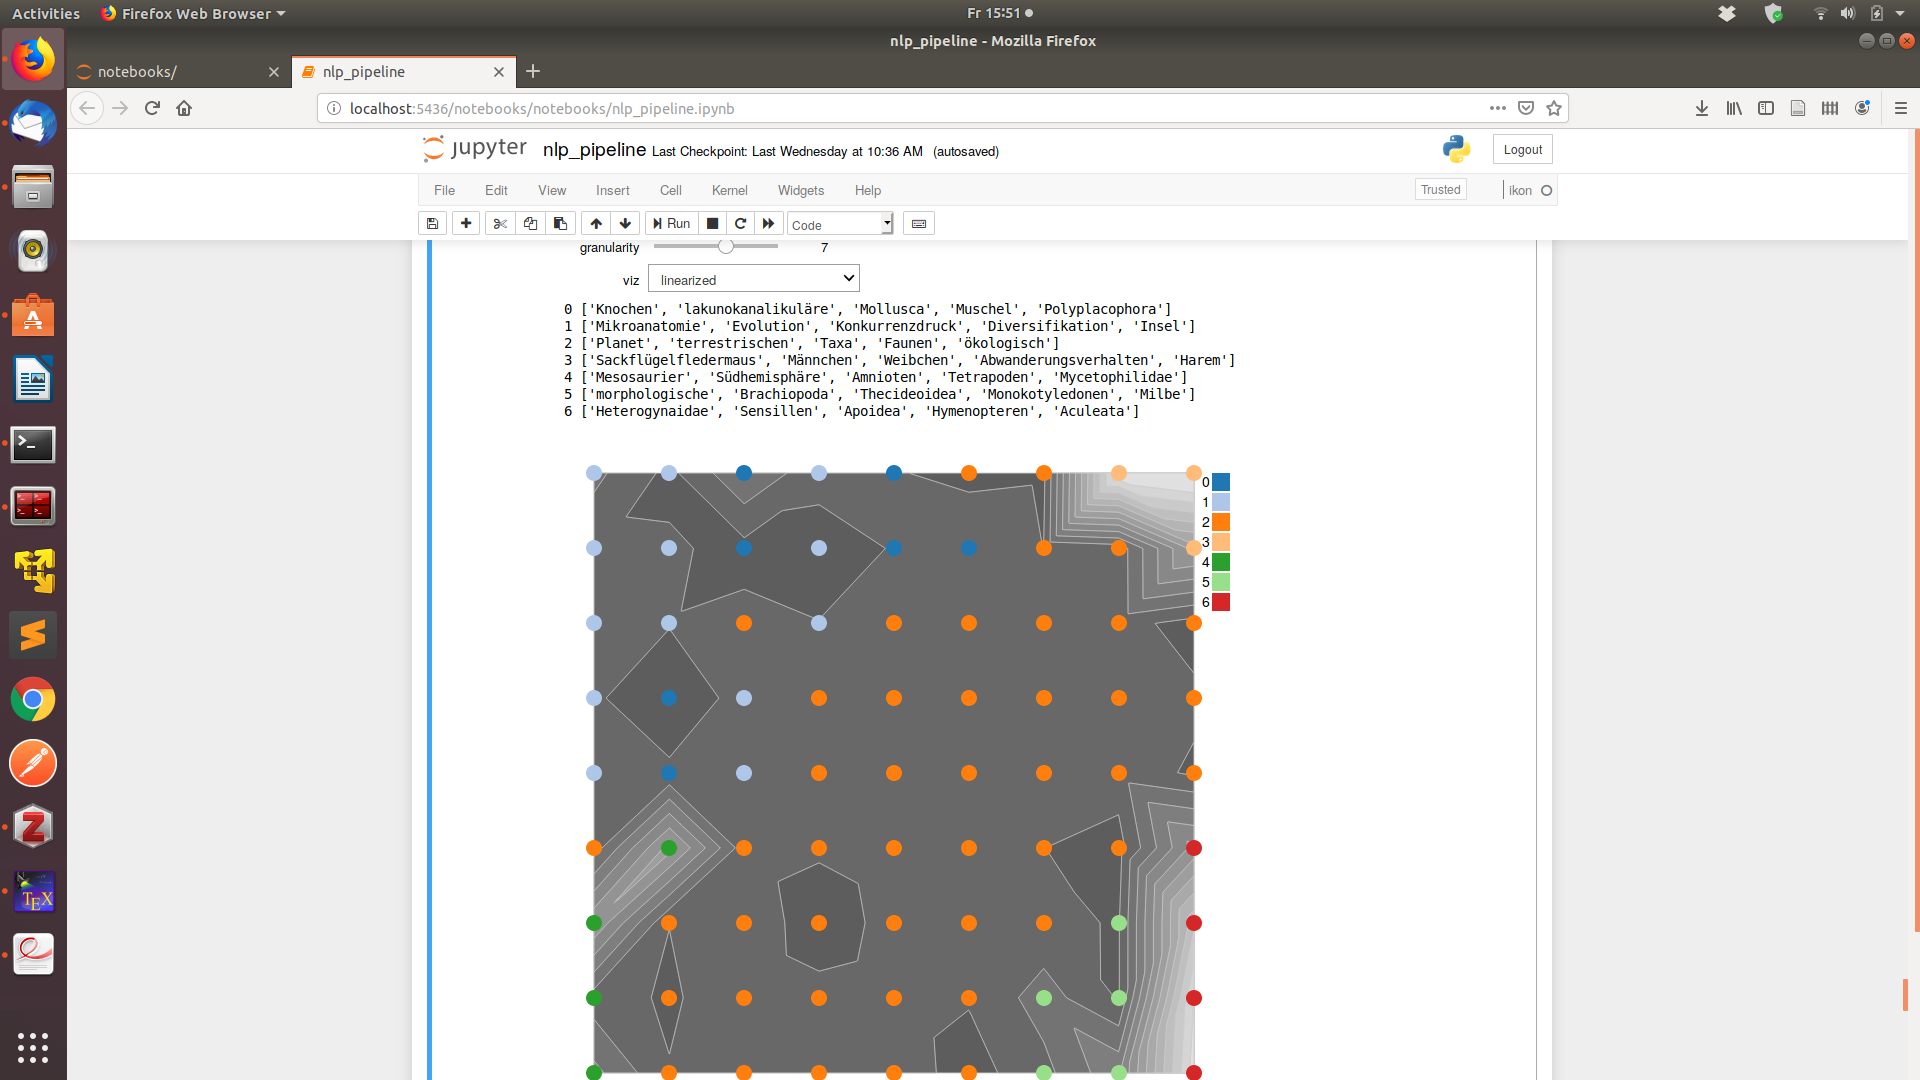
\includegraphics[width=400px]{../chapters/validation/pics/5}
	\caption{\label{pic:step5} Cognitive Walkthrough step 5}
\end{figure}

\begin{figure}[t]
	\centering
	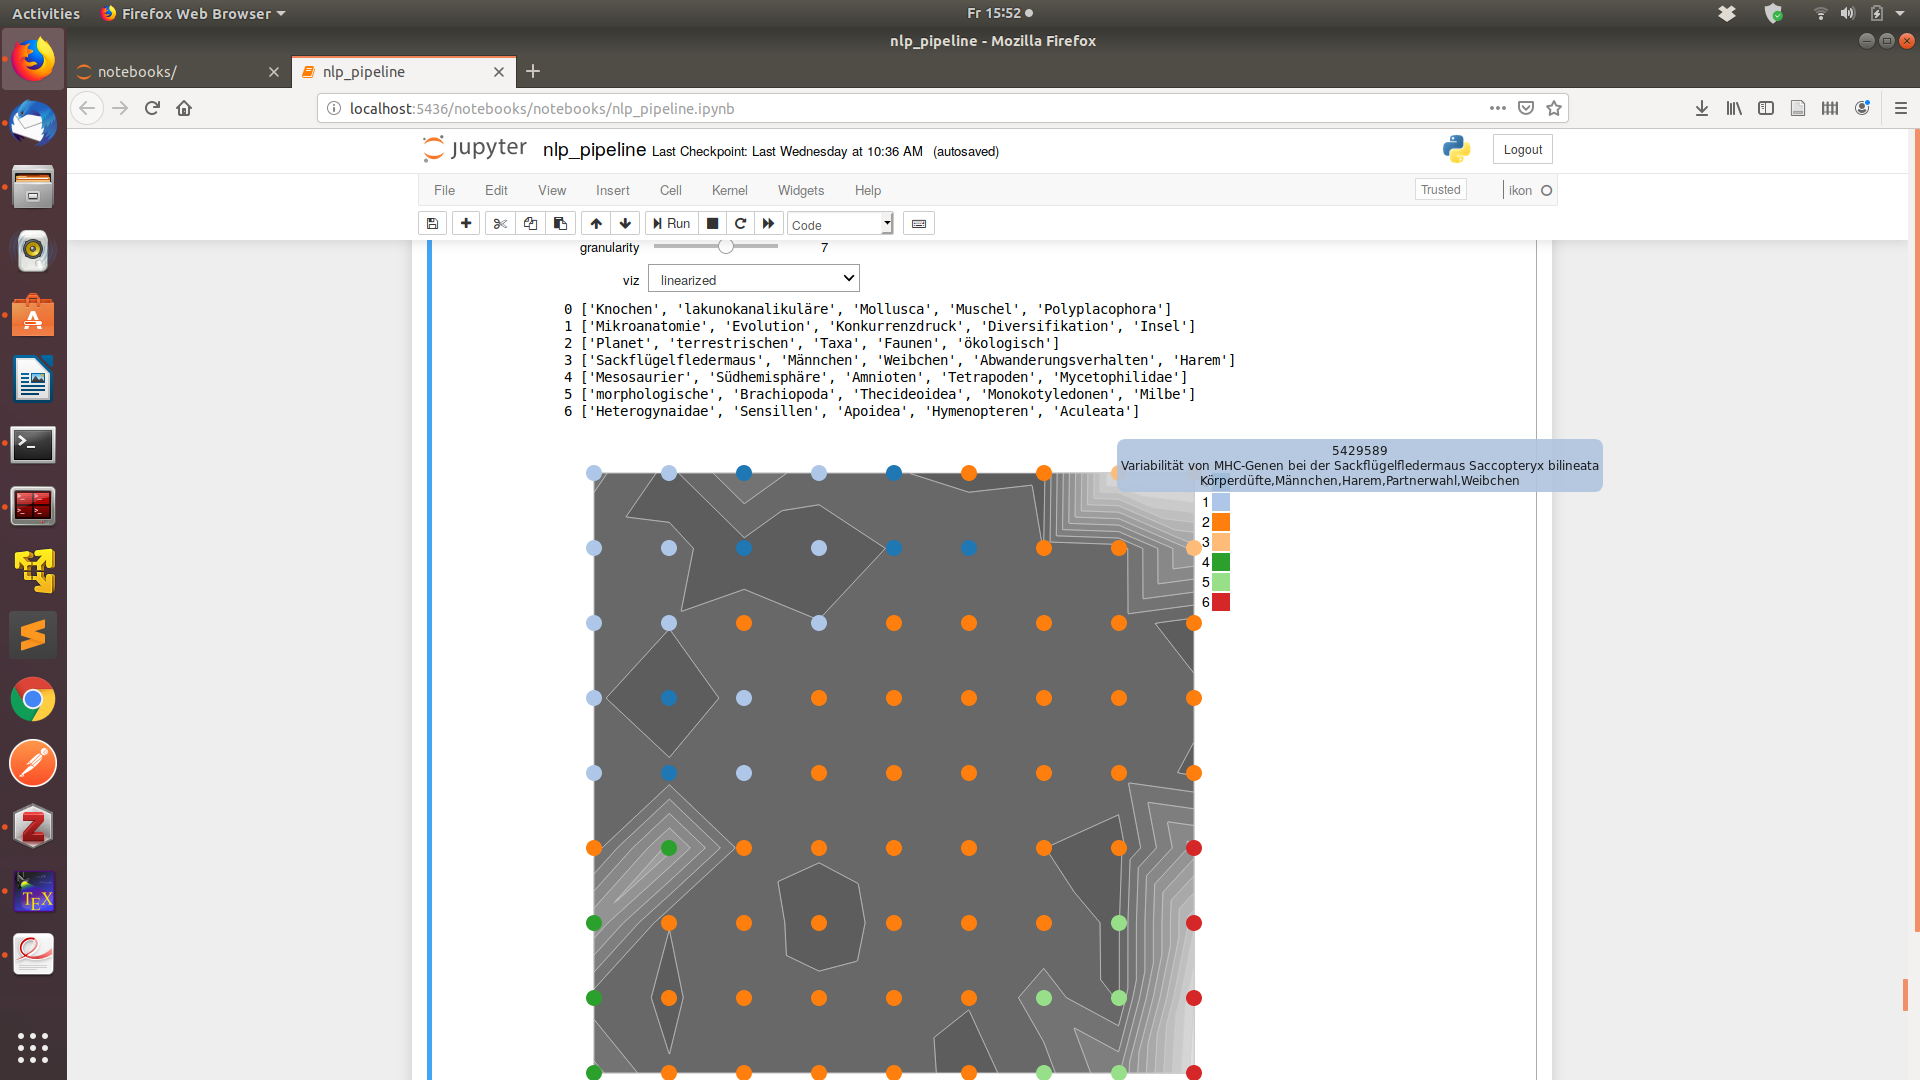
\includegraphics[width=400px]{../chapters/validation/pics/6}
	\caption{\label{pic:step6} Cognitive Walkthrough step 6}
\end{figure}

\begin{figure}[t]
	\centering
	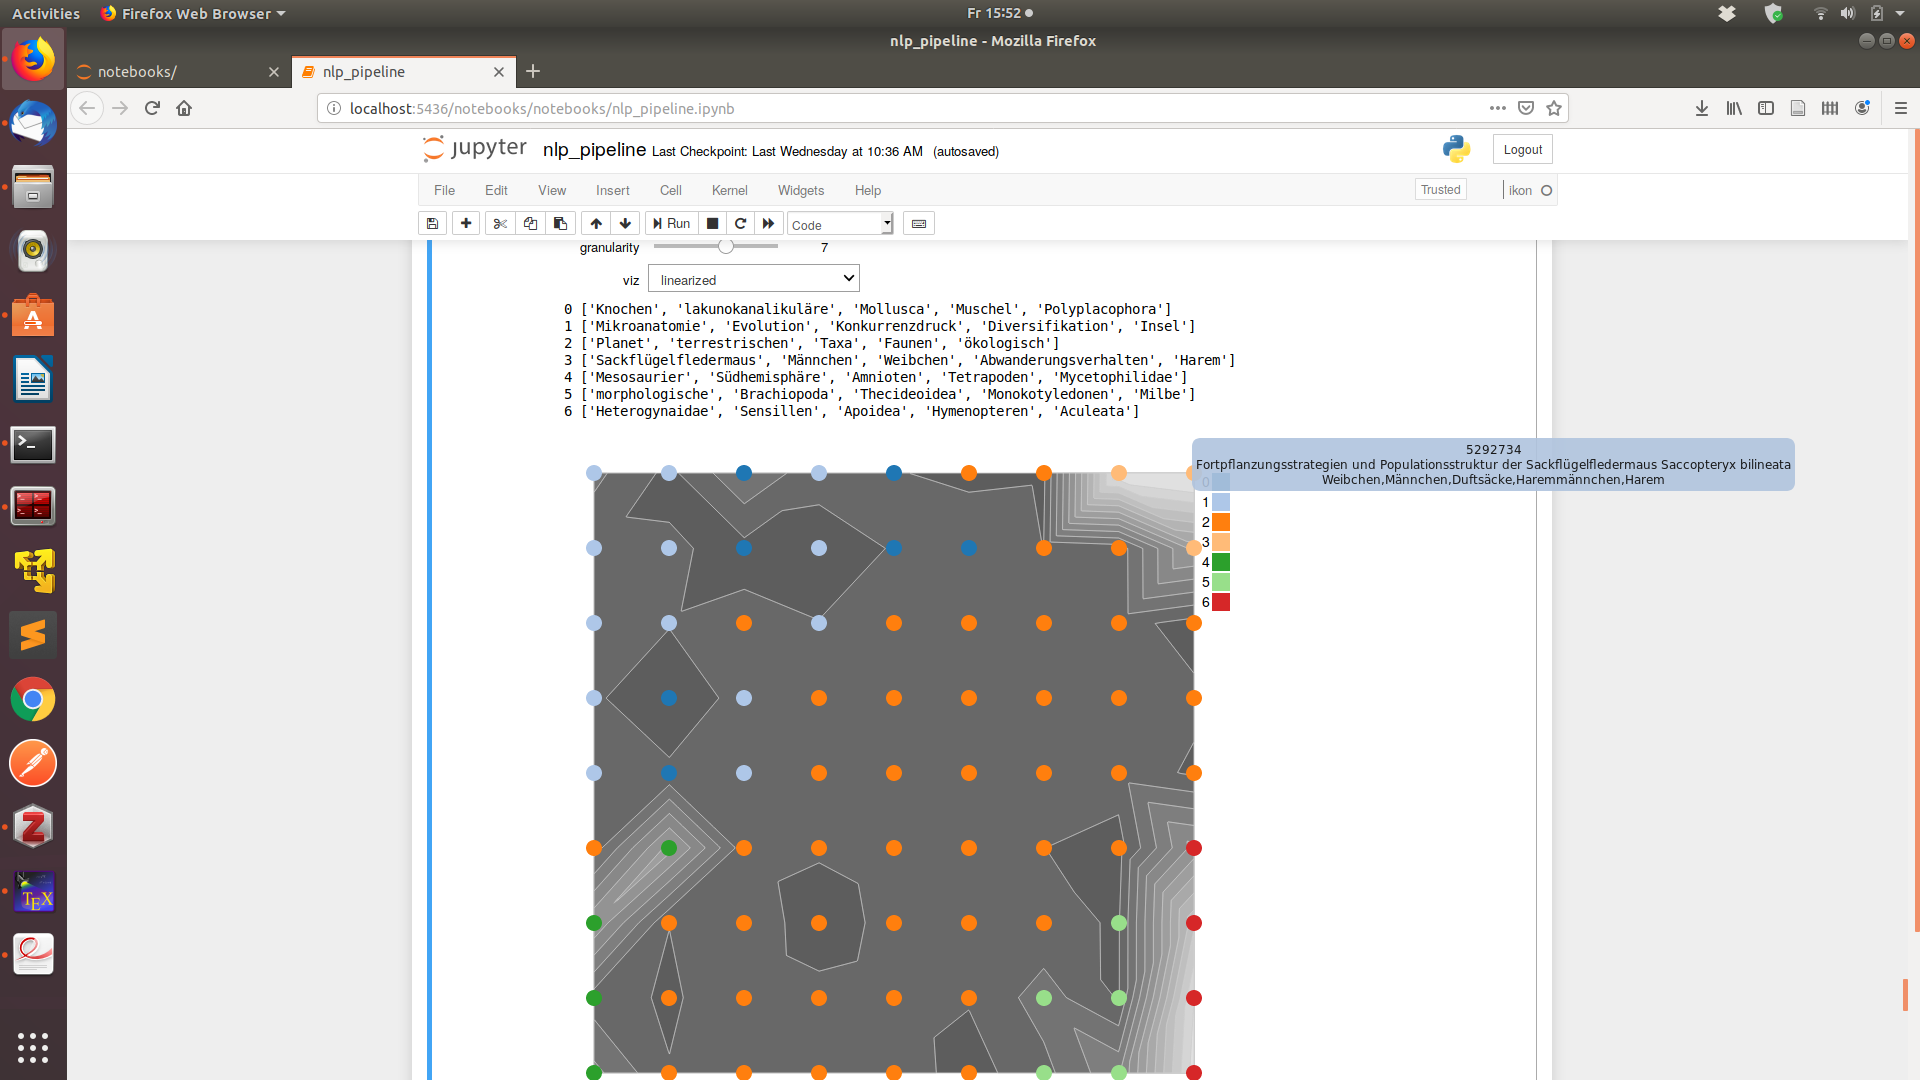
\includegraphics[width=400px]{../chapters/validation/pics/7}
	\caption{\label{pic:step7} Cognitive Walkthrough step 7}
\end{figure}

\begin{figure}[t]
	\centering
	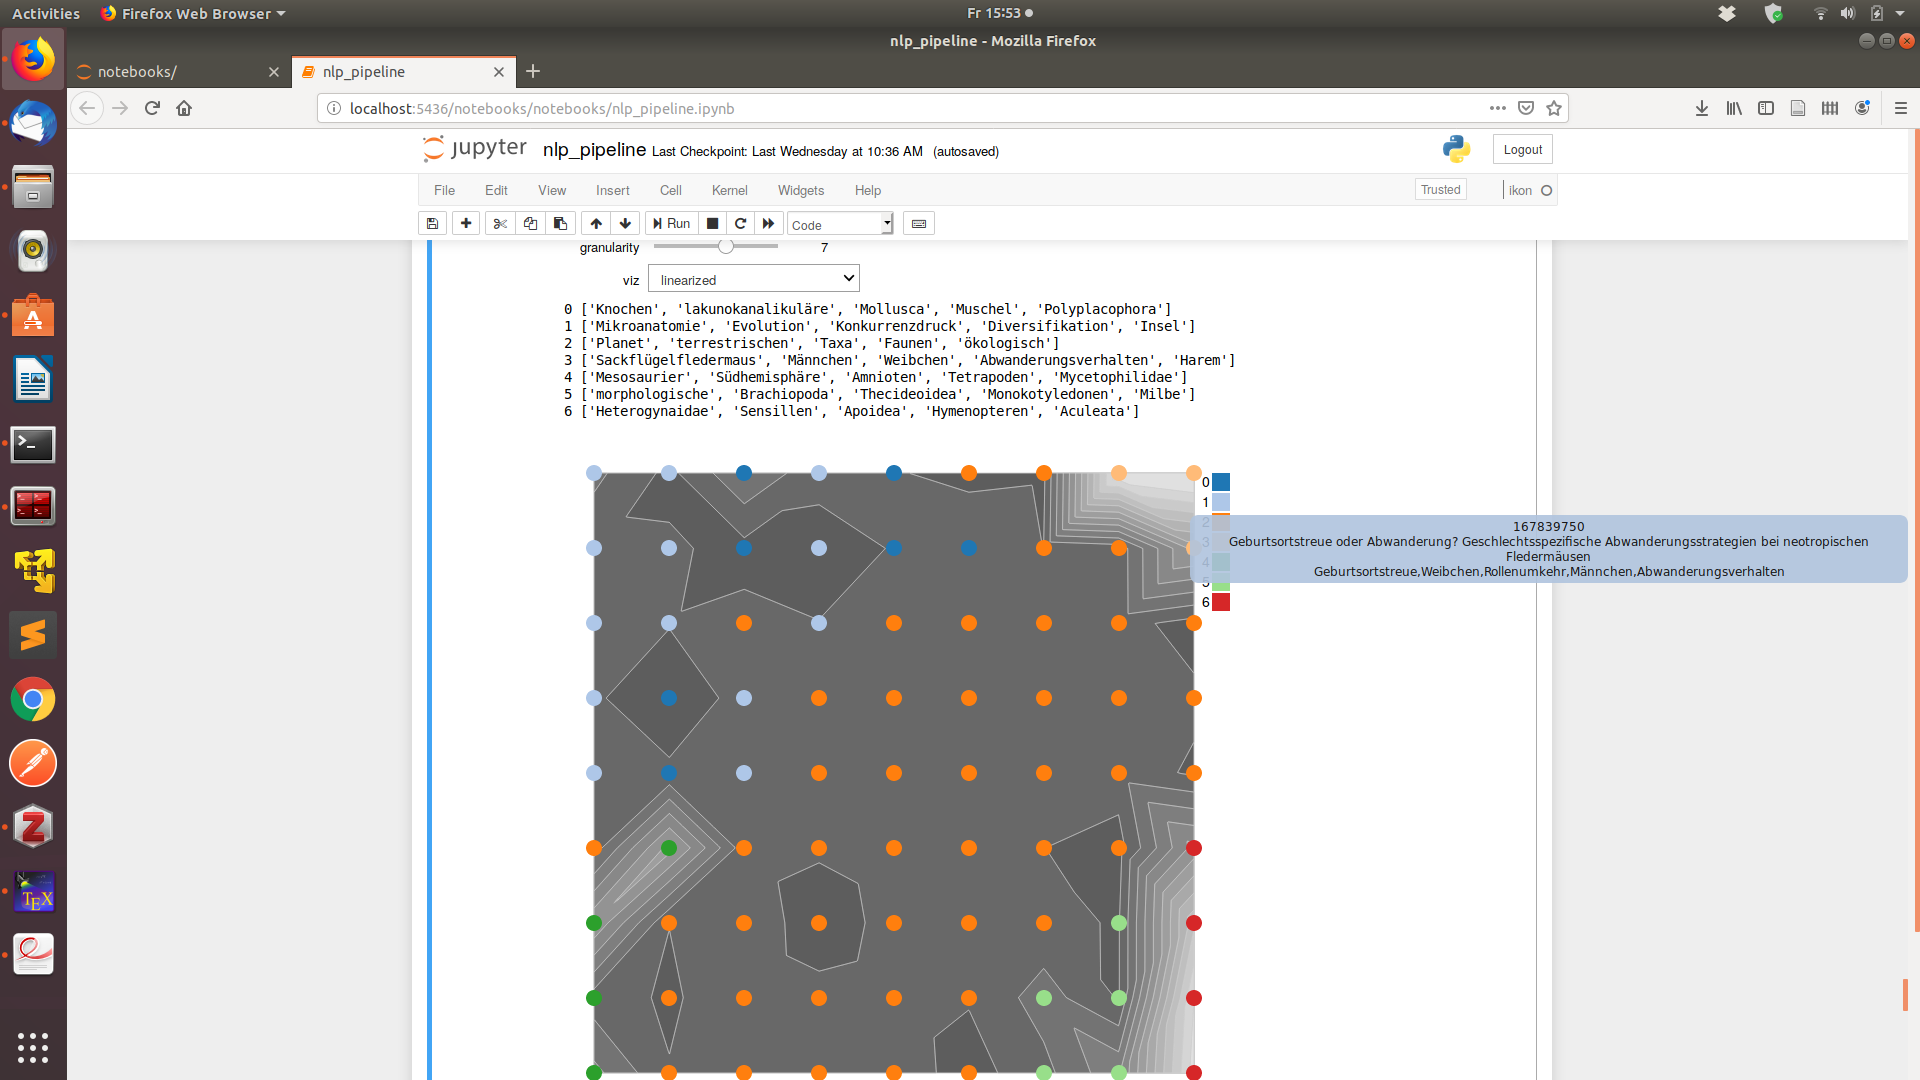
\includegraphics[width=400px]{../chapters/validation/pics/8}
	\caption{\label{pic:step8} Cognitive Walkthrough step 8}
\end{figure}

\begin{figure}[t]
	\centering
	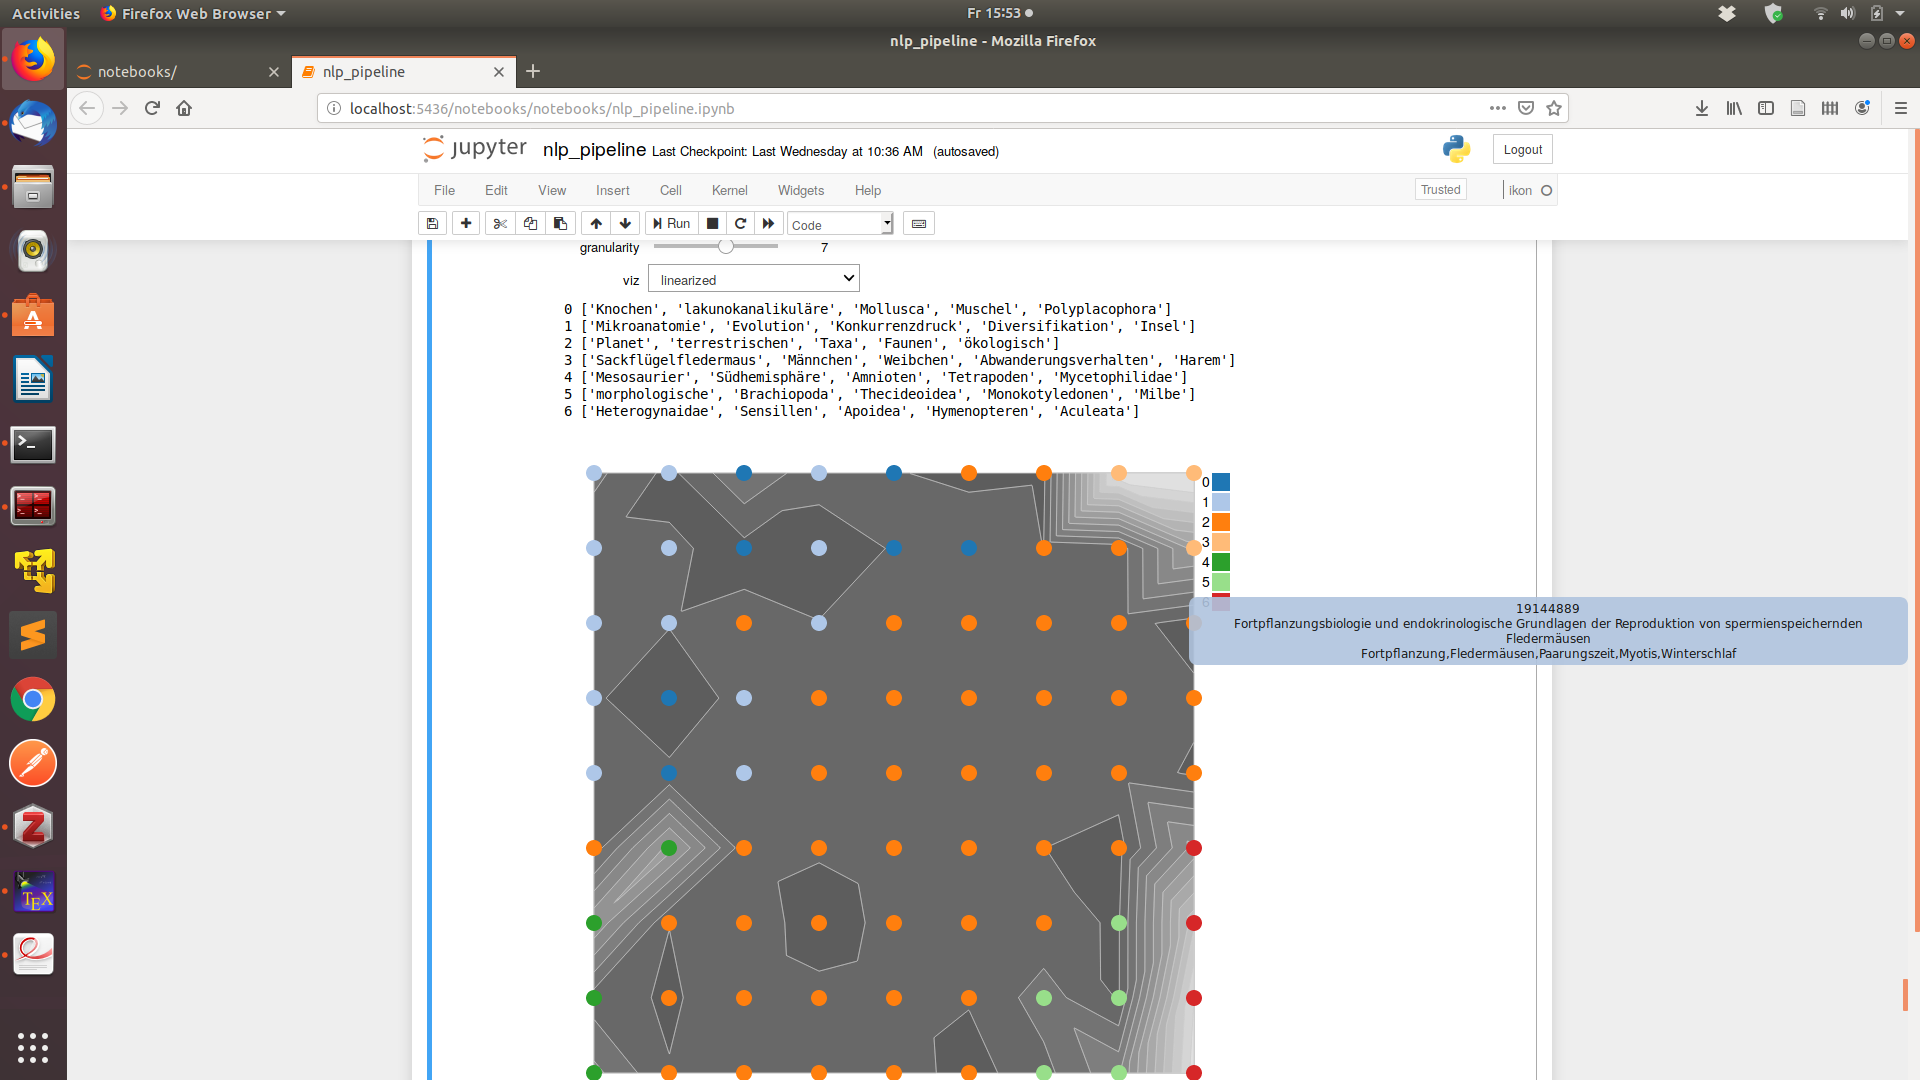
\includegraphics[width=400px]{../chapters/validation/pics/9}
	\caption{\label{pic:step9} Cognitive Walkthrough step 9}
\end{figure}

\begin{figure}[t]
	\centering
	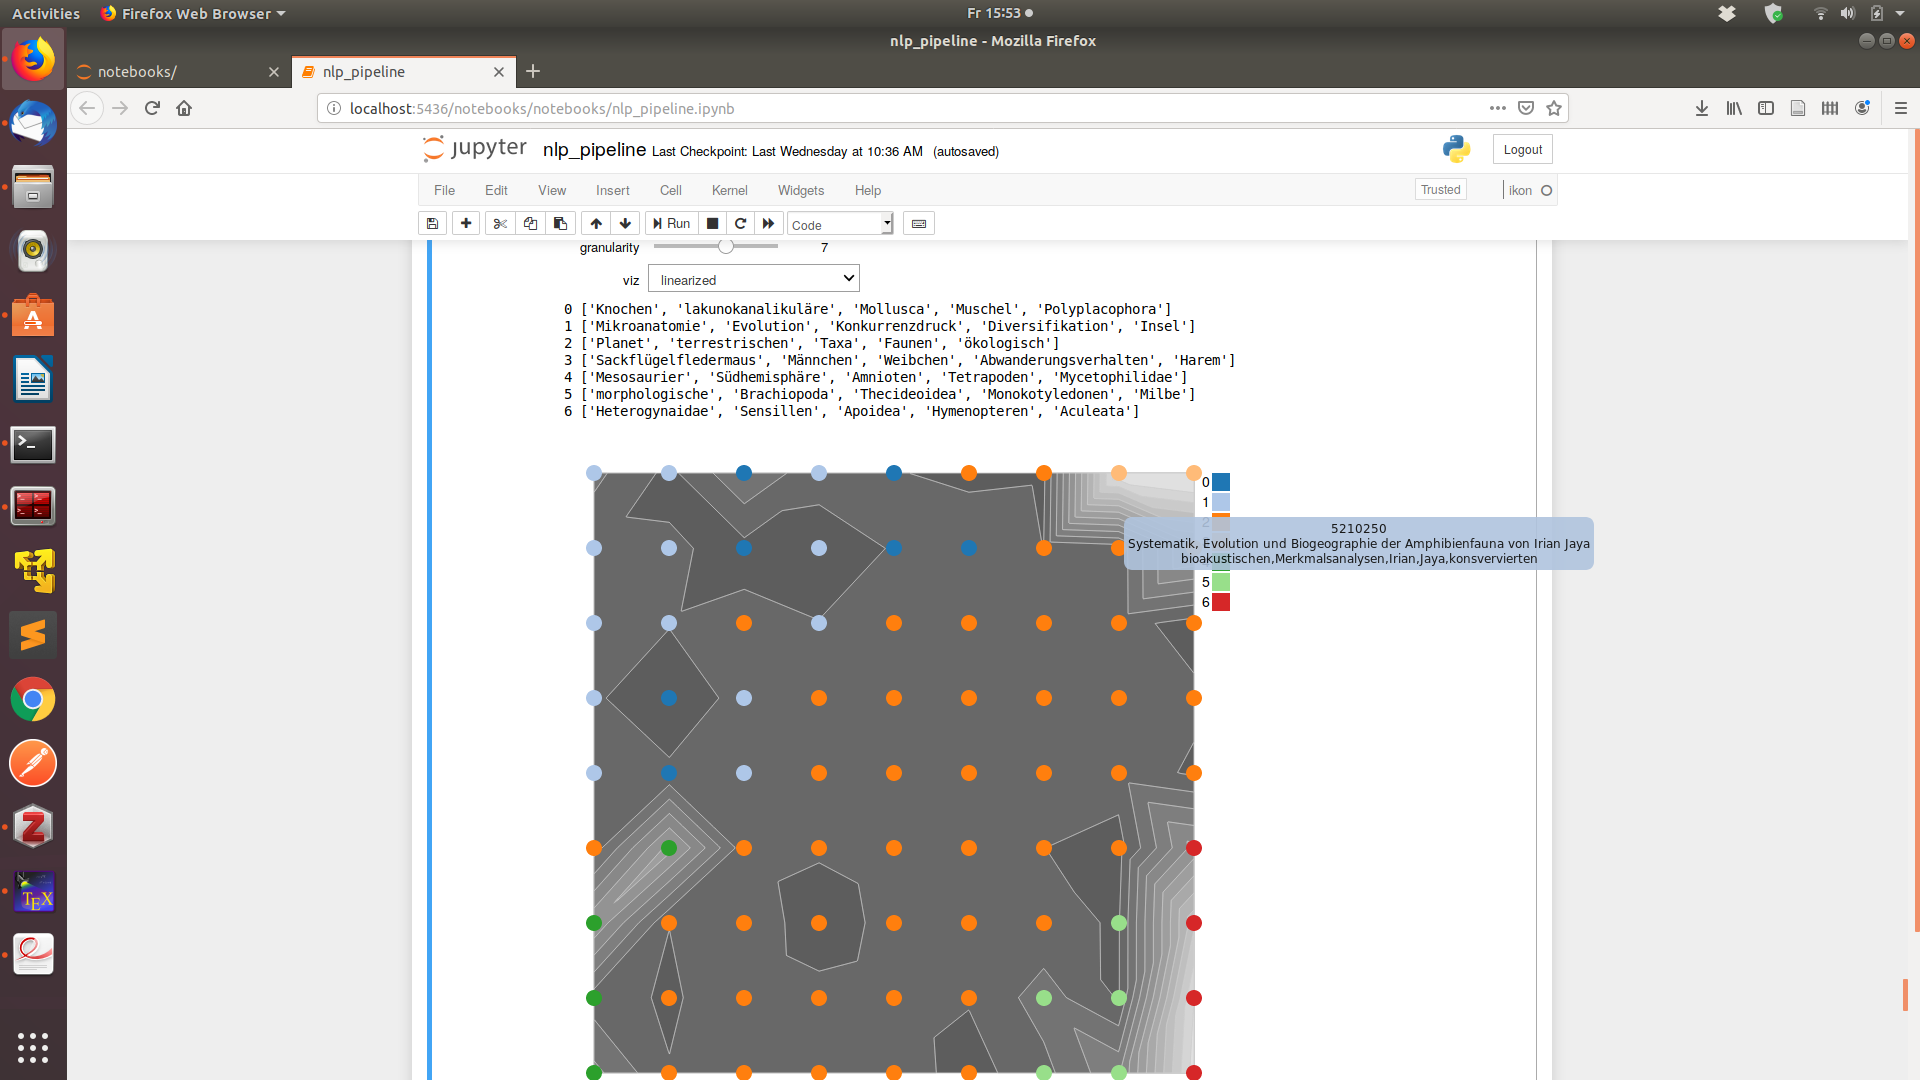
\includegraphics[width=400px]{../chapters/validation/pics/10}
	\caption{\label{pic:step10} Cognitive Walkthrough step 10}
\end{figure} 



%---------------------------------------------------
%----- Bibliography
%---------------------------------------------------
\phantomsection
\addcontentsline{toc}{../chapters/appendix/appendix}{Literatur}
\bibliographystyle{alpha}
\bibliography{../references/thesis/main,../chapters/literature_analysis/data/mapping}


\end{document}